%%%%%%%%%%%%%%%%%%%%%%%%%%%%%%%%%%%%%%%%%%%%%%%%%%%%%%%%%%%%%%%%%%%%%%%%%%%%%%%%
%% Plantilla de memoria en LaTeX para la ETSIT - Universidad Rey Juan Carlos
%%
%% Por Gregorio Robles <grex arroba gsyc.urjc.es>
%%     Grupo de Sistemas y Comunicaciones
%%     Escuela Técnica Superior de Ingenieros de Telecomunicación
%%     Universidad Rey Juan Carlos
%% (muchas ideas tomadas de Internet, colegas del GSyC, antiguos alumnos...
%%  etc. Muchas gracias a todos)
%%
%% La última versión de esta plantilla está siempre disponible en:
%%     https://github.com/gregoriorobles/plantilla-memoria
%%
%% Para obtener PDF, ejecuta en la shell:
%%   make
%% (las imágenes deben ir en PNG o JPG)

%%%%%%%%%%%%%%%%%%%%%%%%%%%%%%%%%%%%%%%%%%%%%%%%%%%%%%%%%%%%%%%%%%%%%%%%%%%%%%%%

\documentclass[a4paper, 12pt]{book}
%\usepackage[T1]{fontenc}

\usepackage[a4paper, left=2.5cm, right=2.5cm, top=3cm, bottom=3cm]{geometry}
\usepackage{times}
\usepackage[utf8]{inputenc}
\usepackage[spanish]{babel} % Comenta esta línea si tu memoria es en inglés
\usepackage{url}
%\usepackage[dvipdfm]{graphicx}
\usepackage{graphicx}
\usepackage{float}  %% H para posicionar figuras
\usepackage[nottoc, notlot, notlof, notindex]{tocbibind} %% Opciones de índice
\usepackage{latexsym}  %% Logo LaTeX
\usepackage{color}
\definecolor{red}{rgb}{1,0,0}
\definecolor{green}{rgb}{0.3,0.6,0.1}
\definecolor{blue}{rgb}{0.2,0.2,0.8}
%\usepackage[dvipsnames]{xcolor}
%\usepackage[usenames]{color} %Textos en color

\title{Integración de una plataforma de telefonía IP}
\author{Javier Estébanez Rodríguez}

\renewcommand{\baselinestretch}{1.5}  %% Interlineado

\begin{document}

\renewcommand{\refname}{Bibliografía}  %% Renombrando
\renewcommand{\appendixname}{Apéndice}

%%%%%%%%%%%%%%%%%%%%%%%%%%%%%%%%%%%%%%%%%%%%%%%%%%%%%%%%%%%%%%%%%%%%%%%%%%%%%%%%
% PORTADA

\begin{titlepage}
\begin{center}
\includegraphics[scale=0.8]{img/URJ_logo_Color_POS.png}

\vspace{1.75cm}

\Large
Grado en Ingeniería en Sistemas Audiovisuales y Multimedia

\vspace{0.4cm}

\large
Curso Académico 2021/2022

\vspace{0.8cm}

Trabajo Fin de Grado

\vspace{2.5cm}

\LARGE
INTEGRACIÓN DE UNA PLATAFORMA DE TELEFONÍA IP

\vspace{4cm}

\large
Autor : Javier Estébanez Rodríguez \\
Tutor : Gregorio Robles Martínez
\end{center}
\end{titlepage}

\newpage
\mbox{}
\thispagestyle{empty} % para que no se numere esta pagina


%%%%%%%%%%%%%%%%%%%%%%%%%%%%%%%%%%%%%%%%%%%%%%%%%%%%%%%%%%%%%%%%%%%%%%%%%%%%%%%%
%%%% Para firmar
\clearpage
\pagenumbering{gobble}
\chapter*{}

\vspace{-4cm}
\begin{center}
\LARGE
\textbf{Trabajo Fin de Grado}

\vspace{1cm}
\large
Integración de una Plataforma de Telefonía IP

\vspace{1cm}
\large
\textbf{Autor :} Javier Estébanez Rodríguez \\
\textbf{Tutor :} Dr. Gregorio Robles Martínez

\end{center}

\vspace{1cm}
La defensa del presente Trabajo Fin de Grado se realizó el día \qquad$\;\,$ de julio de 2022, siendo calificada por el siguiente tribunal:


\vspace{0.5cm}
\textbf{Presidente:}

\vspace{1.2cm}
\textbf{Secretario:}

\vspace{1.2cm}
\textbf{Vocal:}


\vspace{1.2cm}
y habiendo obtenido la siguiente calificación:

\vspace{1cm}
\textbf{Calificación:}


\vspace{1cm}
\begin{flushright}
Fuenlabrada, a \qquad$\;\,$ de julio de 2022
\end{flushright}

%%%%%%%%%%%%%%%%%%%%%%%%%%%%%%%%%%%%%%%%%%%%%%%%%%%%%%%%%%%%%%%%%%%%%%%%%%%%%%%%
%%%% Dedicatoria

\chapter*{}
\pagenumbering{Roman} % para comenzar la numeracion de paginas en numeros romanos
\begin{flushright}
\textit{Dedicado a mis padres y a mi pareja}
\end{flushright}

%%%%%%%%%%%%%%%%%%%%%%%%%%%%%%%%%%%%%%%%%%%%%%%%%%%%%%%%%%%%%%%%%%%%%%%%%%%%%%%%
%%%% Agradecimientos

\chapter*{Agradecimientos}
%\addcontentsline{toc}{chapter}{Agradecimientos} % si queremos que aparezca en el índice
\markboth{AGRADECIMIENTOS}{AGRADECIMIENTOS} % encabezado

Quiero agradecerle a mis hermanos y a mis padres la tremenda y abrumadora paciencia que han tenido conmigo durante toda la carrera y la realización de este proyecto, en especial a mi madre y a sus incansables recordatorios cada vez que pasaba de visita por su casa preguntándome si había empezado ya el TFG. Estoy convencido de que tanto ella como mi padre estarán mucho más contentos de lo que estaré yo (que ya será mucho) cuando por fin lo presente ante el tribunal.

También quiero agradecerle a mis amigos su característica preocupación por el estado de mi título de ingeniero en forma de burlas hacia mi persona, pues me han enseñado indirectamente y de forma totalmente no intencionada a rebajar el estrés y la angustia que sentía al respecto. 
Siguiendo la máxima de ``si no puedes vencerlos únete a ellos'', he acabado por convertirme en un auténtico icono del auto-vilipendio en clave de humor.

Quiero dar las gracias también a mi pareja por apoyarme siempre, por ayudarme a centrarme, por soportarme cuando los nervios me atenazaban y por introducir en mi cabeza poco a poco, siguiendo los pasos mi madre, la idea de finalizar definitivamente lo que me quedaba pendiente para conseguir mi titulación.

Por último, también quiero agradecer a mis compañeros de trabajo por su gran involucración y amabilidad a la hora de explicarme cada cosa que no entendía durante la realización del proyecto. He aprendido mucho con ellos y espero poder seguir haciéndolo.
%%%%%%%%%%%%%%%%%%%%%%%%%%%%%%%%%%%%%%%%%%%%%%%%%%%%%%%%%%%%%%%%%%%%%%%%%%%%%%%%
%%%% Resumen

\chapter*{Resumen}
%\addcontentsline{toc}{chapter}{Resumen} % si queremos que aparezca en el índice
\markboth{RESUMEN}{RESUMEN} % encabezado

El objetivo de esta Trabajo Fin de Grado es presentar una solución de colaboración \emph{on-premise} basada en Cisco UCS para el alojamiento de una infraestructura de telefonía IP, servicios de mensajería y Contact Center.

El sistema consiste principalmente de una centralita que gestionará la lógica de las llamadas de VoIP (Voice over Internet Protocol) con tecnología Cisco basada en un Call Manager y el protocolo SIP (Session Initiation Protocol).
Para hacerlo posible, se ha preparado un entorno de virtualización con la tecnología VMWare, que alojará las máquinas virtuales de la solución.

Este tipo de estructura está pensado para atender las necesidades de varias empresas (en paralelo) en cuestión de atención telefónica. La lógica que pueden esconder los distintos elementos de la arquitectura ofrece un sinfín de posibilidades, de manera que se puede llegar a realizar una gestión muy eficiente y personalizada.

%La inclusión de scripts en el Contact Center ofrece posibilidades como la aparición de una locución de bienvenida con opciones de marcado, el almacenamiento en una base de datos de las respuestas de una encuesta de satisfacción, servicios de enrutado de llamadas según demanda y asignación de colas o de agente basado en sus habilidades, entre muchas otras.
En un mundo cada vez más digitalizado, las empresas se ven obligadas a ofrecer un soporte técnico remoto ya sea telefónicamente, por chat o mediante correo electrónico. En este ámbito, la asistencia telefónica constituye una gran opción que permite mejorar la comunicación y eficiencia en la resolución de problemas, consiguiendo así un mayor grado de satisfacción en el cliente y convirtiéndose a su vez en un importante criterio de evaluación a la hora de elegir la contratación de un servicio/producto.

Empresas como Cisco, Skype o Mitel (entre otros) son grandes referentes en la implementación de estos servicios, que además permiten la comunicación interna entre trabajadores de la misma empresa sin inferir en un sobrecoste.

%%%%%%%%%%%%%%%%%%%%%%%%%%%%%%%%%%%%%%%%%%%%%%%%%%%%%%%%%%%%%%%%%%%%%%%%%%%%%%%%
%%%% Resumen en inglés

\chapter*{Summary}
%\addcontentsline{toc}{chapter}{Summary} % si queremos que aparezca en el índice
\markboth{SUMMARY}{SUMMARY} % encabezado

The main purpose of this memory is to present an on-premise collaboration solution based on Cisco UCS technology to host an IP telephony infrastructure, messaging services and Contact Center.

This system consists mainly of a switchboard which will manage the logic of the VoIP (Voice over Internet Protocol) calls with Cisco tehcnology based on Call Manager and SIP protocol (Session Initiation Protocol). To achieve this goal, a virtualization enviroment has been disposed with VMWare technology, hosting the virtual machines all over the solution.

This kind of structure is meant to attend the parallel needs of many enterprises in terms of telephone support. The logic that may hide behind the different elemments of the architecture offers an endless range of possibilities, so that an eficient and personalized management can be achieved.

In a world more and more digitalized, the enterprises has been forced to offer a remote technical support, which can be telephonic, by chat or by e-mail. In this scope, the telephone assistance can establish a great option to improve the communication and eficiency on issues resolution, reaching a higher degree in customer satisfaction and becoming a highly valuable criteria when hiring a service or product.

Many enterprises as Cisco, Skype or Mitel are huge referents on the integration of these services, which can also allow the internal communication between workers of the company without incurring a cost overrun.

%%%%%%%%%%%%%%%%%%%%%%%%%%%%%%%%%%%%%%%%%%%%%%%%%%%%%%%%%%%%%%%%%%%%%%%%%%%%%%%%
%%%%%%%%%%%%%%%%%%%%%%%%%%%%%%%%%%%%%%%%%%%%%%%%%%%%%%%%%%%%%%%%%%%%%%%%%%%%%%%%
% ÍNDICES %
%%%%%%%%%%%%%%%%%%%%%%%%%%%%%%%%%%%%%%%%%%%%%%%%%%%%%%%%%%%%%%%%%%%%%%%%%%%%%%%%

% Las buenas noticias es que los índices se generan automáticamente.
% Lo único que tienes que hacer es elegir cuáles quieren que se generen,
% y comentar/descomentar esa instrucción de LaTeX.

%%%% Índice de contenidos
\tableofcontents
%%%% Índice de figuras
\cleardoublepage
%\addcontentsline{toc}{chapter}{Lista de figuras} % para que aparezca en el indice de contenidos
\listoffigures % indice de figuras
%%%% Índice de tablas
%\cleardoublepage
%\addcontentsline{toc}{chapter}{Lista de tablas} % para que aparezca en el indice de contenidos
%\listoftables % indice de tablas


%%%%%%%%%%%%%%%%%%%%%%%%%%%%%%%%%%%%%%%%%%%%%%%%%%%%%%%%%%%%%%%%%%%%%%%%%%%%%%%%
%%%%%%%%%%%%%%%%%%%%%%%%%%%%%%%%%%%%%%%%%%%%%%%%%%%%%%%%%%%%%%%%%%%%%%%%%%%%%%%%
% INTRODUCCIÓN %
%%%%%%%%%%%%%%%%%%%%%%%%%%%%%%%%%%%%%%%%%%%%%%%%%%%%%%%%%%%%%%%%%%%%%%%%%%%%%%%%

\cleardoublepage
\chapter{Introducción}
\label{sec:intro} % etiqueta para poder referenciar luego en el texto con ~\ref{sec:intro}
\pagenumbering{arabic} % para empezar la numeración de página con números

\section{Presentación de la solución}
\label{sec:seccion}

El objetivo de esta Trabajo Fin de Grado es presentar una solución de colaboración \emph{on-premise} basada en Cisco UCS para el alojamiento de una infraestructura de telefonía IP, servicios de mensajería y Contact Center.
La implementación de esta solución se ha ideado con el objetivo de instalar un sistema de Contact Center en un cliente que dé soporte a varias empresas.
Se pretende que varios agentes gestionen simultáneamente las llamadas de dichas empresas, pudiendo atender indistintamente llamadas de varios de estos orígenes.

De forma paralela, se ha provisto de un servicio de presencia (estado online, ausente, ocupado\ldots) y de mensajería interna mediante el aplicativo Finesse, apoyado en Cisco Jabber.
Mientras que Jabber proveerá del servicio de presencia, voz y monitorización silenciosa de las llamadas, Finesse será la interfaz gráfica que verá el agente, pudiendo entre otras cosas pausar y transferir llamadas o entrar en conferencias.

Adicionalmente, se ha configurado un software de terceros para la grabación de las llamadas. Desde dicho software se pueden escuchar las grabaciones y organizarlas mediante filtros, de manera que su exportación sea más controlada y proporcione datos para estadísticas.



\section{Contexto personal}
%\label{sec:seccion}
En verano de 2021 estuve plenamente implicado en un proyecto de VoIP en la empresa en la actualmente trabajo que me supuso un enorme reto por su complejidad, diseño inicial desde cero y las exigentes ``deadlines'' impuestas por el cliente.

Estas circunstancias me obligaron a investigar mucho por mi cuenta sin realmente tener la posibilidad de poder apoyarme inicialmente en perfiles más completos de mi empresa al encontrarse de vacaciones.
Como suelen decir, y aunque a menudo suponga un gran esfuerzo, a veces hay que ``pegarse con ello'' para aprender y sacar las cosas adelante.
Aún contando con ayuda de mis compañeros en fases más avanzadas del proyecto, mi dedicación ha sido plena desde el inicio hasta el final, y sigue siéndolo en la inclusión de mejoras en la actualiad.

La idea de que este proyecto fuera mi Trabajo Fin de Grado me pareció idónea por su contenido tan cercano a los conocimientos adquiridos en mi grado. A su vez me ha ayudado a hacer un análisis más a bajo nivel de la implementación, que me permitirá interiorizar con más precisión cada elemento configurado y su importancia dentro de la arquitectura, y así poder replicarlo en futuros proyectos.

\section{Contexto}
%\label{sec:seccion}
Tras vivir recientemente una situación límite en muchos aspectos con la pandemia de la COVID-19, el modelo de negocio actual se ha visto obligado a adaptarse para integrar el trabajo remoto en el día a día a consecuencia de las medidas de restricción sanitarias que están teniendo lugar.
Estas circunstancias han favorecido en gran medida el crecimiento de las soluciones de telefonía IP y colaboración, que ya habían sido objeto de estudio previamente por consultoras de análisis de mercados, %como \textit{Market and Research} o \textit{Global Market Insights}
arrojando unos resultados prometedores de crecimiento entre los años 2017 y 2021 y previendo la continuación de dicha tendencia en los próximos años~\cite{researchandmarkets}.

Si bien hay distintas soluciones de telefonía IP pretenden lograr el mismo objetivo, podemos distinguir entre los dos métodos de integración que se pueden llevar a cabo actualmente:
\begin{itemize}
  \renewcommand{\theenumi}{\alph{enumi}}
  \item \underline{On premise} o local, donde el montaje de la arquitectura se hace habitualmente en las propias instalaciones de la empresa, la cual necesita comprar, instalar y mantener el hardware. Los costes iniciales son grandes y requiere personal cualificado para su gestión, pero proporcionan un control completo y autónomo de la solución. Además, son más seguros al no tener elementos fuera de la red local por lo que el flujo de comunicación se queda dentro de la red propia.  

  \item \underline{Cloud} o en la nube, que puede ser pública o privada. La gestión y mantenimiento de la arquitectura se hace remotamente, de lo que generalmente se encarga el proveedor. Son servicios más baratos, más facilmente escalables y su puesta en marcha es mucho más rápida y sencilla, aunque impide un control total de la configuración al encontrarse supeditada a las posibilidades que ofrezca el proveedor.
\end{itemize}

Para el despliegue de estas tecnologías podemos distinguir entre empresas que ofrecen productos propios frente a empresas que ofrecen productos basados en tecnología de código abierto (Asterix por ejemplo), o empresas que ofrecen productos \emph{on premise}\footnote{\url{https://www.gartner.com/reviews/market/contact-center-infrastructure}} frente a otras más incipientes en el mercado actual que ofrecen soluciones en cloud\footnote{\url{https://www.gartner.com/reviews/market/contact-center-as-a-service}}. Cabe hacer mención a varias empresas que ofrecen servicios de CC (Contact Center)  líderes en el sector, y representadas en años consecutivos en los famosos cuadrantes de Gartner (como se puede observar en la Figura~\ref{figura:fig_gartner}):
\begin{itemize}
  \item \textbf{Cisco.} Entre los muchos mercados en los que se encuentra, dedica al de VoIP gran parte de su atención y esfuerzo.   

  \begin{itemize}
    \item \emph{UCCX}: Unified Contact Center Express es la aplicación de centro de atención al cliente on premise que se presenta en esta memoria. Una herramienta muy potente bajo el renombre de una marca con gran reconocimiento mundial.
    \item \emph{Webex}: Muy expandida en Europa y Norte América. Ofrece un despliegue de CC en la nube con gran rapidez y flexibilidad en necesidades puntuales por sobrecarga, entre otros.
  \end{itemize}  

  \item \textbf{Mitel}: Su solución \emph{MiContact Center Business}\footnote{\url{https://www.mitel.com/es-es/productos/aplicaciones/contact-center/micontact-center-business}}, a menudo de la mano con la centralita de Call Manager MiVoice MX-ONE, es una plataforma de nivel profesional para la gestión de experiencia del cliente omnicanal, diseñada para las empresas orientadas al cliente.

  \item \textbf{Genesys}: Referente mundial en soluciones de CC y experiencia de cliente omnicanal. Presente en valoraciones Gartner de CCaaS (Contact Center as a Service) y UCaaS (Unified Communications as a Service)~\cite{gartner:_magic_quadrant}.
\end{itemize}

\begin{figure}[h]
  \centering
  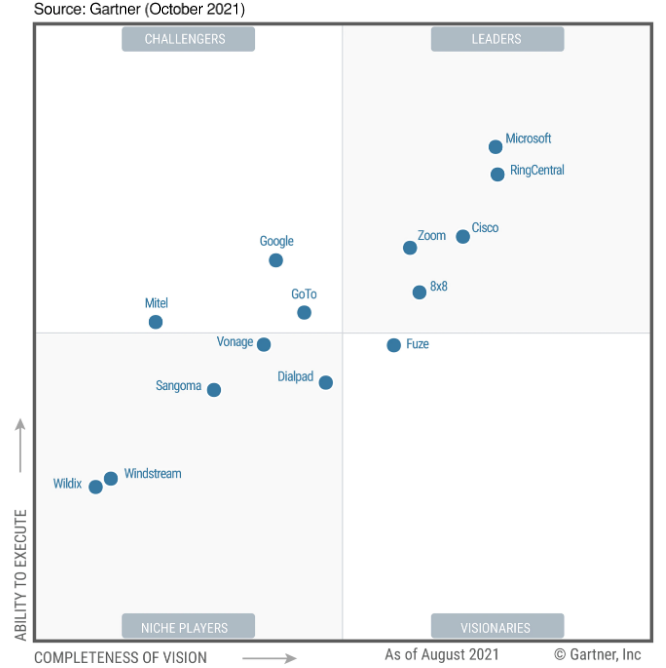
\includegraphics{img/fig_gartner_2021}
  \caption{Cuadrante mágico para UCaaS 2021. Fuente: Gartner.}
  \label{figura:fig_gartner}
\end{figure}

En el mercado VoIP actual se está valorando cada vez más la sencillez de instalación, la interfaz, la facilidad de uso y la integración con múltiples herramientas de trabajo, además del siempre presente interés por el mayor ahorro posible dentro de unos estándares mínimos de calidad. Estos ``requisitos'' han ocasionado que emerjan soluciones de colaboración principalmente en cloud destinadas a ese propósito, pero que no ofrecen servicios de CC. Entre ellas, caben destacar dos archiconocidas en España:
\begin{itemize}
  \item \textbf{Microsoft Teams} es la herramienta que se usa actualmente en esta universidad. Tiene una interfaz amigable, sencilla, potente y con garantías de una empresa con gran trayecto andado en este ámbito, pues podría decirse que Teams es el resultado de la evolución y muerte de Skype.  

  \item \textbf{Zoom}. No ha sido hasta la reciente pandemia que esta empresa ha ganado mayor renombre. Muy utilizada por la educación pública de España y cada vez más empleada en empresas para satisfacer sus necesidades de comunicación, reuniones, chat, y seminarios web.
\end{itemize}
  

\section{Estructura de la memoria}
%\label{sec:seccion}

A continuación se muestra la estructura que tendrá la memoria:
\begin{itemize}
  \item En el primer capítulo se presenta el contexto personal, motivaciones de presentación de este proyecto y una pequeña introducción del contexto global.
  
  \item  En el segundo capítulo se muestran las necesidades, objetivos y planificaciones que se llevaron a cabo para abordar el trabajo.  

  \item El capítulo 3 refleja las tecnologías empleadas en la consecución del diseño, haciendo hincapié en las referentes a la comunicación vía VoIP.
  
  \item El capítulo 4 muestra la arquitectura y los flujos de comunicación entre los elementos del sistema.  

  \item Por último, el capítulo 5 contiene las conclusiones sacadas de esta experiencia.
\end{itemize}

% {\footnotesize
% \begin{verbatim}
%     From gaurav at gold-solutions.co.uk  Fri Jan 14 14:51:11 2005
%     From: gaurav at gold-solutions.co.uk (gaurav_gold)
%     Date: Fri Jan 14 19:25:51 2005
%     Subject: [Mailman-Users] mailman issues
%     Message-ID: <003c01c4fa40$1d99b4c0$94592252@gaurav7klgnyif>

%     Dear Sir/Madam,
%     How can people reply to the mailing list?  How do i turn off
%     this feature? How can i also enable a feature where if someone
%     replies the newsletter the email gets deleted?
%     Thanks

%     From msapiro at value.net  Fri Jan 14 19:48:51 2005
%     From: msapiro at value.net (Mark Sapiro)
%     Date: Fri Jan 14 19:49:04 2005
%     Subject: [Mailman-Users] mailman issues
%     In-Reply-To: <003c01c4fa40$1d99b4c0$94592252@gaurav7klgnyif>
%     Message-ID: <PC173020050114104851057801b04d55@msapiro>

%     gaurav_gold wrote:
%     >How can people reply to the mailing list?  How do i turn off
%     this feature? How can i also enable a feature where if someone
%     replies the newsletter the email gets deleted?

%     See the FAQ
%     >Mailman FAQ: http://www.python.org/cgi-bin/faqw-mm.py
%     article 3.11
% \end{verbatim}
% }

%%%%%%%%%%%%%%%%%%%%%%%%%%%%%%%%%%%%%%%%%%%%%%%%%%%%%%%%%%%%%%%%%%%%%%%%%%%%%%%%
%%%%%%%%%%%%%%%%%%%%%%%%%%%%%%%%%%%%%%%%%%%%%%%%%%%%%%%%%%%%%%%%%%%%%%%%%%%%%%%%
% OBJETIVOS %
%%%%%%%%%%%%%%%%%%%%%%%%%%%%%%%%%%%%%%%%%%%%%%%%%%%%%%%%%%%%%%%%%%%%%%%%%%%%%%%%

\cleardoublepage % empezamos en página impar
\chapter{Objetivos} % título del capítulo (se muestra)
\label{chap:objetivos} % identificador del capítulo (no se muestra, es para poder referenciarlo)

\section{Objetivo general} % título de sección (se muestra)
\label{sec:objetivo-general} % identificador de sección (no se muestra, es para poder referenciarla)

El objetivo general de este proyecto consiste en idear e implementar una solución de centro de atención al cliente telefónico basado en VoIP y a su vez cubrir las necesidades de comunicación interna de una empresa. 


\section{Objetivos específicos}
\label{sec:objetivos-especificos}

Para lograr que el diseño sea adecuado, he definido una serie de objetivos específicos que se desean alcanzar:

\begin{itemize}

  \item Instalación física de los servidores y demás elementos en los CPDs (Centro de Procesamiento de Datos) correspondientes, es decir, trasladarlos a sus ubicaciones finales en las instalaciones del cliente.
  
  \item Instalar los aplicativos de software en los servidores. Proveer de configuraciones de red a los equipos y realizar las instalaciones de los sistemas operativos necesarias.

  \item Conseguir que el sistema permita mensajería y llamadas a través de la extension interna. Como primeras pruebas de funcionamiento, hay que comprobar que al menos las llamadas internas se cursan y los mensajes llegan entre agentes.
  
  \item Adaptar la herramienta al teletrabajo. Para ello, es necesario permitir que los agentes se puedan registrar contra la centralita (de ahora en adelante ``Call Manager'') de forma remota, sin dependencia de estar conectado a una VPN.   

  \item Integrar el elemento que actúa de gestor de agentes en llamadas entrantes: el Contact Center. Configurar la lógica para que se asigne el agente idóneo con relacion a la consulta recibida.

  \item Configurar e integrar el elemento que actúa de borde en la red para que gestione las llamadas entrantes y salientes a la PSTN.
  
  \item Redundar geográficamente la solución en dos o más CPDs, de manera que el servicio siga activo y funcionando aunque haya una caída en cualquiera de las ubicaciones físicas, ya sea de tensión o de internet, o por cualquier factor no previsto.

  \item Integrar un elemento de grabación de llamadas, tanto entrantes como salientes. Dicho elemento permitirá también filtrar y exportar grabaciones.
  
  \item Monitorizar los elementos del sistema, de modo que un equipo de soporte técnico pueda detectar si hay alarmas que requieran atención.
\end{itemize}

\section{Planificación temporal}
\label{sec:planificacion-temporal}

Esta memoria refleja de forma didáctica y aproximada lo que fue todo el diseño y puesta en producción de un proyecto real que llevé a cabo en la empresa en la que estoy actualmente empleado. 
A mediados de verano de 2021 llegó a mi departamento un proyecto con unas fechas muy justas. Trataba de una actualización desde cero de un sistema de atención al cliente que daba soporte telefónico a varias empresas. De forma resumida, el cliente cambiaba de marca y había que hacer un traslado de una arquitectura similar a la que tenían en ese momento a unos nuevos servidores, pero más actualizada y con más elementos. Por la tipología de este escenario, se pudieron reutilizar algunos elementos, como scripts con la lógica para despachar llamadas entre los agentes disponibles, los nombres y extensiones de los agentes, los grupos de captura y grupos de salto de llamadas, entre otros.

En aquel entonces no había gente suficiente para cubrir todas las tareas que había que llevar a cabo, y yo no tenía la suficiente experiencia como para montar de cero todo un sistema de telefonía IP, de modo que tuve que estar 8 horas diarias durante unas dos semanas estudiando cada elemento, cada flujo de comunicacion y la configuracion de todos los equipos. Pasadas esas dos semanas llegaron los equipos físicos a las oficinas de Madrid, así que ahí comenzaron mis tareas de configuración inicial de los equipos. 
Una vez realizada, se pudieron mandar los equipos físicos a los CPDs del cliente y comenzar con las configuraciones de forma remota. Para esta labor conté con ayuda de dos consultores de redes y telefonía experimentados, de manera que de forma guiada pude participar al 100\% en cada tarea prevista.

De forma un poco resumida, puedo decir que la totalidad del proyecto ocupó unos dos meses de trabajo intensivo, más otros dos meses de correcciones y añadidos que quedaron pendientes. Detallo los pequeños hitos que se iban cumpliendo:
\begin{itemize}
  \item Preparación individual para el diseño y puesta en marcha.
  
  \item Reuniones de planificación con el cliente, reuniones diarias de seguimiento y reuniones extraordinarias de resolución de conflictos o discrepancias en la organización. Diseños iniciales, revisiones y remates posteriores a dichos diseños.

  \item Inventariado de todos los elementos, tanto físicos como virtuales. Datos de acceso, diagramas de la arquitectura, números de serie, IPs de cada máquina y licencias, localizaciones físicas en los racks\footnote{Armario con base y estructura metálica pensado para alojar sistemas informáticos}, flujos de servicio con sus protocolos y traducciones de DNS (\emph{Domain Name System}), entre otros. Se aprovechó la semana que tardaron los equipos en llegar y ser instalados en el cliente para comenzar con estos trabajos. Dichos documentos se fueron actualizando también a medida que se fue avanzando en el proyecto.

  \item Configuraciones de los equipos. En el Capítulo 4 hablaré más detenidamente de cada elemento y su papel en el entorno, pero de forma resumida podemos decir que el Call Manager (CUCM) y el Contact Center (UCCX) acapararon la mayor parte del tiempo en configuraciones, seguidos muy de cerca por el Session Border Controller (SBC). Durante aproximadamente un mes se estuvieron haciendo configuraciones, en jornada laboral a tiempo completo, con horas extras como medida de urgencia.

  \item Primera puesta en producción básica. Debido a los plazos tan ajustados, se lanzó a producción el sistema con una funcionalidad básica para ``salir del paso''. Posteriormente, se fueron añadiendo más configuraciones, como el sistema de grabación, la redundancia, grupos de salto de llamadas y certificados.

  \item Pulido de las funcionalidades y resolución de problemas. No hay nada mejor para aprender como tener incidencias y no encontrar las soluciones tras cuantiosas horas de búsqueda y estudio de flujos a bajo nivel. Entre varias incidencias de la integración que había que resolver, estuvimos atascados durante dos semanas tratando de solventar un problema en la aceptación de dígitos de marcado en la locución de bienvenida, también llamada Interactive Voice Response (IVR).
  
  \item Como la puesta en producción se hizo para atender a una empresa en concreto, hubo que ir integrando al resto de empresas contratantes del servicio de atención telefónica del cliente.
  
  \item A día de hoy se siguen haciendo mejoras y acualizaciones del entorno, pero me centaré en los detalles del proyecto inicial para la presentación de esta memoria.
\end{itemize}



%%%%%%%%%%%%%%%%%%%%%%%%%%%%%%%%%%%%%%%%%%%%%%%%%%%%%%%%%%%%%%%%%%%%%%%%%%%%%%%%
%%%%%%%%%%%%%%%%%%%%%%%%%%%%%%%%%%%%%%%%%%%%%%%%%%%%%%%%%%%%%%%%%%%%%%%%%%%%%%%%
% ESTADO DEL ARTE %
%%%%%%%%%%%%%%%%%%%%%%%%%%%%%%%%%%%%%%%%%%%%%%%%%%%%%%%%%%%%%%%%%%%%%%%%%%%%%%%%

\cleardoublepage
\chapter{Estado del arte}
\label{chap:estado}

El aumento del ancho de banda con el paso de los años y la naturaleza actual del ``always-on'' en términos de constante conectividad a la red, han ido permitiendo a la tecnología VoIP ir tomando su lugar en sustitución a los teléfonos tradicionales. Así mismo, la mejora de la transmisión de paquetes y su fiabilidad en el orden de llegada ha sido un paso importante para su adopción como sistema principal de comunicación en empresas. Este avance ha proporcionado ventajas importantes, como el aprovechamiento del cableado interno de red de datos para el envío de voz, infiriendo en un gasto muy reducido del coste de llamadas o incluso reduciéndolo a cero.

El estándar VoIP consigue un encapsulamiento de la voz para enviarlo por circuitos no conmutados, creando un circuito virtual y aprovechándolo para el envío de múltiples conversaciones paquetizadas y en flujos independientes, puediendo además aprovechar al máximo los recursos que le ofrece el medio, por ejemplo cuando en una conversación se produce un silencio y esos recursos sobrantes se reutilizan para ``alimentar'' al resto de flujos activos. 
No así es el caso de la red de telefonía pública (PSTN), que reserva los recursos y crea un circuito físico punto a punto cuando se establece una llamada y en el tiempo que dura la misma, impidiendo un aprovechamiento eficiente.

En este aspecto, las plataformas internas de telefonía IP conectadas a la red pública para permitir llamadas entrantes y salientes, comunmente llamadas PABX (\emph{Private Automatic Branch Exchange}), se han ido expandiendo, convirtiéndose en un elemento imprescindible en muchos casos. 

\section{Tecnologías actuales}
\label{sec:tecnologias-actuales}

La tecnologías más usadas actualmente en telefonía IP son los protocolos SIP (Session Initiation Protocol) y H.323, diseñados ambos en 1996.
\begin{itemize}
  \item  \textbf{SIP}. Protocolo creado y gestionado por la Internet Engeneering Task Force (IETF), organización internacional abierta de normalización. SIP se basa en el establecimiento de llamadas P2P, donde los usuarios o agentes inician la sesión. Su flujo de peticiones es muy similar al de HTTP, y soporta la negociación de parámetros, codificación y y envío de datos por protocolo RTP/RTCP.
  \item \textbf{H.323}. Creado por la Unión Internacional de Telecomunicaciones (ITU) y diseñado, al igual que SIP, para proveer sesiones de comunicación audiovisual a través de la red (RTP). Su funcionamiento es muy parecido al de SIP, pero con pequeñas diferencias.
  \\
  \begin{figure}[h]
    \centering
    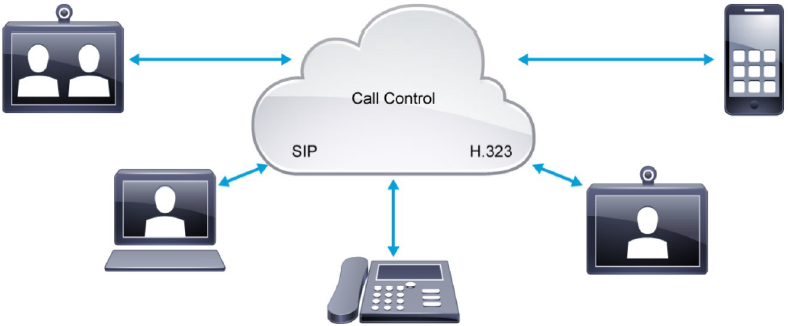
\includegraphics{img/fig_diagrama_simple_collab}
    \caption{Esquema simple de VoIP}
    \label{figura:fig_diagrama_simple_collab}
  \end{figure}
\end{itemize}

Los protocolos RTP (\emph{Real-time Transport Protocol}) y RTCP (\emph{Real Time Control Protocol}) involucrados en las sesiones SIP y H.323 son los responsables de la transmisión fiable de voz y vídeo a travez de Internet. RTP es el encargado de la transmisión de datos, mientras que RTCP proporciona informacion de control complementaria al flujo de datos RTP. Debido a su naturaleza, este protocolo utiliza UDP (\emph{User Datagram Protocol}) a nivel de transporte, pues necesita un flujo constante de datos y gran ancho de banda para reducir el tiempo de envío de los paquetes~\cite{cisco:_video}.

Para estas labores de envío de datos juegan un papel fundamental los códecs. El objetivo de un códec de audio es comprimir la señal para reducir la cantidad de bits a enviar, de manera que en la recepción se pueda descomprimir y obtener una señal lo más parecida posible a la original. Este proceso de codificar/decodificar facilita el envío de datos para conseguir una mayor cantidad de paquetes aprovechando el ancho de banda disponible.

En la actualidad existen cientos de códecs, muchos de ellos propietarios. SIP usa Session Description Protocol (SDP), que define en la cabecera de los mensajes de una conversación SIP todos los códeds soportados, los cuales están identificados por una cadena de caracteres y pueden ser registrados por cualquier persona. Esto hace que SIP pueda funcionar con cualquier códec.

H.323 se caracteriza sin embargo por requerir que cada códec esté registrado y estandarizado de forma centralizada, hecho que repercute en pequeñas desarrolladoras y universidades pues muchos traen propiedad intelectual; no existen los códecs sub-28.8Kb/s gratis que puedan ser usados en un sistema H.323. Por todo ello, y gracias a su facilidad de implementación y adaptabilidad a la naturaleza evolutiva de Internet, SIP está ganando gran populariad, siendo el protocolo de elección en las soluciones de Cisco y Microsoft, entre otros. Además su  ``interfaz'' amigable al lenguaje humano permite hacer \emph{debugging} con mayor facilidad y legibilidad.
Ambos protocolos son muy usados no obstante.
\\

\begin{table} [h]
  \begin{center}
    \begin{tabular}{| c | c |}
    \hline
    \textbf{H.323} & \textbf{SIP} \\ \hline
    Extenso, complejo y rígido & Modular, flexible y extensible\\\hline
    Buena interoperabilidad por su rigidez & Fácilmente adaptable a nuevas funcionalidades\\\hline
    Codificación en binario & Codificación en ASCII \\\hline
    Direcciones por \emph{host} o \#tlf & Direcciones por URLs \\ \hline
    Q.931 sobre TCP & SIP sobre TCP/UDP \\\hline
    \end{tabular}
    \label{tabla:SIPvsH.323}
    \caption{Comparativa entre SIP y H.323}
  \end{center}
\end{table}

\subsection{SIP}
\label{sec:sip}

Tomando como referencia protocolos con un gran recorrido y un buen historial de evolución como HTTP y SMTP, SIP~\cite{johnston2009sip} ha basado la lógica de sus flujos de comunicación en una estructura de petición -$>$ respuesta. Este flujo de de comunicación Resquest/Response (como se puede ver en la Figura~\ref{figura:fig_phones}) utiliza los llamados \emph{métodos} SIP, compuestos por un grupo reducido de sencillas cabeceras con nombres muy intuitivos.

\begin{figure}[h]
  \centering
  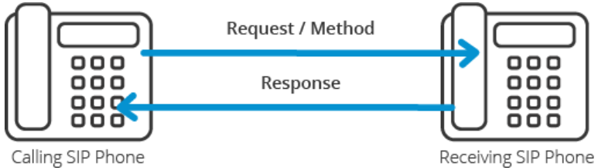
\includegraphics{img/fig_phones}
  \caption{Comunicación vía SIP entre dos terminales}
  \label{figura:fig_phones}
\end{figure}

De forma resumida, se puede decir que las más importantes son:
\begin{itemize}
  \item \textbf{INVITE}. Petición con la que un agente invita a otro a una sessión telefónica.
  \item \textbf{ACK}. Mensaje de respuesta de confirmación de recepción de la petición INVITE.
  \item \textbf{REGISTER}. Registra contra un servidor SIP la dirección listada en la cabecera ``To''.
  \item \textbf{BYE}. El cliente corta la conexión.\\
\end{itemize}

SIP generalmente trae consigo un protocolo de descripción de sesión, llamado SDP, cuyo propósito es transmitir información acerca de los streams de media para ayudar a los participantes a recolectar información sobre una llamada. Proporciona información acerca de la sesión, como el nombre y propósito de la sesón, información del medio, protocolos, formatos de códec, tiempo e información del transporte. Además, posee una estructura corta y visual con descripción textual, con entradas del tipo $<$type$>$ = $<$value$>$.

SDP permite a un participante consultar toda esta información antes de aceptar la invitación, de manera que puede decidir si unirse o no a la llamada, o determinar de qué manera y en qué momento unirse si decide hacerlo.

En la Figura~\ref{figura:fig_sip_flow} se puede ver un ejemplo de flujo SIP entre dos teléfonos IP. Entre ambos \emph{endpoints} se encuentra un servidor SIP, que se encarga de registrar sus direcciones y reenviar las peticiones si tuviera también el papel de proxy. En este contexto, se pueden distinguir cuatros procesos:
\begin{enumerate}
  \item Proceso de registro de los agentes contra el servidor SIP para que otros agentes puedan localizarlos. Este proceso se realiza cuando los usuarios encienden su dispositivo, y así se quedan hasta que reciben o realizan una llamada.
  \item Proceso de invitación a sesión, el \emph{Tinder} de las comunicaciones VoIP. Agente1 manda la invitación al servidor SIP con la dirección de Agente2 en la cabecera ``To:''. El servidor SIP busca dicha dirección en su base de datos y una vez hay match, reenvía la petición a Agente2. Este elemento intermedio envía inmediatamente una respuesta 100 Trying a Agente1 para no comience retransmisiones de la petición INVITE. Si Agente2 acepta la llamada, comienza la transmisión de la petición 180 Ringing, a la que seguirá una respuesta 200 OK. Una vez Agente1 recibe el 200 OK, envía una petición ACK, dando luegar al siguiente proceso.
  \item Establecimiento de sesión. Comienza la transmisión punto a punto de paquetes vía RTP, ya sea para audio o vídeo. El servidor SIP no tiene cabida en este escenario, pues se ha creado una conversación privada entre los dos usuarios.
  \item Cuando un agente desea colgar, envía una petición BYE al servidor, el cual la retransmitirá a Agente2. A Agente2 no le quedará otra que aceptar la finalización de sesión y devolver una respuesta 200 OK, retransmitida a Agente1.
\end{enumerate}

\begin{figure}[h]
  \centering
  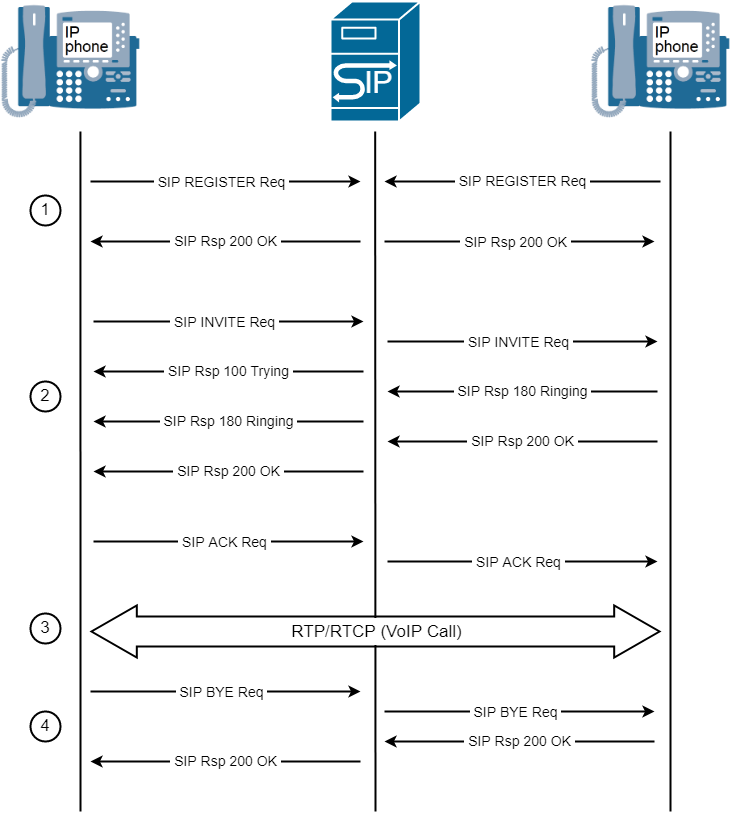
\includegraphics{img/fig_sip_flow}
  \caption{Flujo básico SIP}
  \label{figura:fig_sip_flow}
\end{figure}

\subsection{Tecnologías complementarias}
\label{sec:tecnologias-complementarias}
Junto a SIP, Cisco usa un protocolo propietario de control de terminal desarrollado en 1998, nombrado Skinny Call Control Protocol (SCCP) y comúnmente llamado Skinny, para la comunicación entre el Call Manager y clientes ligeros, tales como los teléfonos IP (figura ~\ref{figura:fig_skinny}). La labor de este protocolo ha quedado relegada a una cantidad pequeña de tareas, como la especificacion de recrusos de media o la comunicación opcional con equipos analógicos. Actualmente, todos los nuevos teléfonos IP funcionan con SIP.

\begin{figure}[h!]
  \centering
  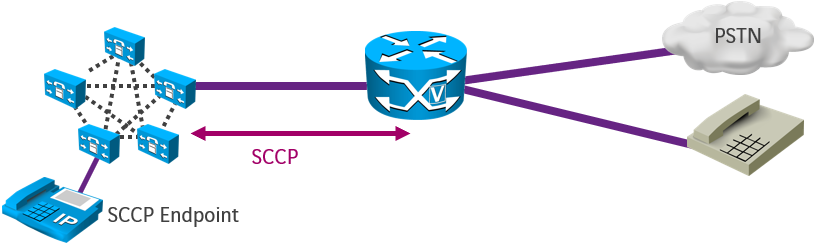
\includegraphics{img/fig_skinny}
  \caption{Flujo de comunicación por SCCP}
  \label{figura:fig_skinny}
\end{figure}

%%%%%%%%%%%%%%%%%%%%%%%%%%%%%%%%%%%%%%%%%%%%%%%%%%%%%%%%%%%%%%%%%%%%%%%%%%%%%%%%
%%%%%%%%%%%%%%%%%%%%%%%%%%%%%%%%%%%%%%%%%%%%%%%%%%%%%%%%%%%%%%%%%%%%%%%%%%%%%%%%
% DISEÑO E IMPLEMENTACIÓN %
%%%%%%%%%%%%%%%%%%%%%%%%%%%%%%%%%%%%%%%%%%%%%%%%%%%%%%%%%%%%%%%%%%%%%%%%%%%%%%%%

\cleardoublepage
\chapter{Diseño e implementación}

De acuerdo a los contratos legales establecidos entre mi empresa (ejecutora del proyecto) y el cliente (receptora), no me está permitido hacer una reproducción de la solución con un detalle exacto, pero sí puedo definir de forma aproximada una arquitectura funcional similar, intentando reflejar todas mis tareas ejecutadas durante la instalación.

\section{Arquitectura general}
\label{sec:arquitectura}

En la figura ~\ref{figura:fig_arquitectura} se muestra un esquema simplificado de la solución, presentando cuatro zonas delimitadas~\cite{cisco:_ccna}.

Empezando desde arriba, la primera zona representa la red pública de telefonía (PSTN), desde la que una persona puede realizar una llamada desde su teléfono móvil o fijo al número de atención al cliente definido para la entrada al sistema. También tenemos una pequeña nube representando el \emph{Busines to Business}, que en este caso son empresas con su propia red de telefonía privada conectadas a la solución de este proyecto mediante un elemento intermedio de control de fronteras: el SBC.

En la segunda zona, sobrepasando el primer borde de control, podemos diferenciar dos capas imaginarias:
\begin{itemize}
  \item Capa de conectividad, donde están ubicados el Gateway de voz y el SBC, ambos elementos físicos. Sus funciones serán enrutar las llamadas hacia la PSTN (a través del Gateway) y enviar las llamadas a los clientes ubicados en las redes privadas de los clientes (a través del SBC).
  \item Capa de servicios, donde se encuentran los servidores físicos que almacenan las máquinas virtuales de estos elementos. Sus funciones serán aplicar, entre otras, toda la lógica de gestión de llamadas entrantes y salientes, la configuración necesaria de interconexionado entre máquinas o las grabaciones de usuarios. El elemento más importante aquí es el Call Manager, que interactúa directamente con el resto de elementos.
\end{itemize}

En la tercera zona, delimitada por dos firewalls y llamada también Zona Desmilitarizada (DMZ), se encuentra un servidor proxy propietario de Cisco con funciones especiales, ya que es el elemento que hace posible el login a la plataforma desde ubicaciones externas a la red privada por parte de los agentes. Esta zona está especialmente diseñada para alojar proxys en su interior, pues tiene la característica de permitir tráfico hacia el exterior pero bloquearlo hacia la red interna. Podría decirse que es como el jardín de una casa, donde se pueden colocar ciertos objetos, pero los de mayor valor se guardan dentro.

Por último, al otro lado del firewall externo, se encuentra la red de Internet. Los agentes se encuentran en esta zona y hacen login a la plataforma desde su domicilio o desde su oficina de trabajo.

\section{Diagrama general}
\label{sec:diagrama}
Los elementos implicados en la solución son los siguientes:
\begin{itemize}
  \item \textbf{Call Manager}. Al ser una solucón redundada, necesitará tener un elemento \emph{master} y otro \emph{slave}.
  \item \textbf{Cisco Unified Presence}. Servidores de presencia, serán \emph{slaves} del Call Manager \emph{master}.
  \item \textbf{Jabber}. Cliente Cisco para llamadas, videoconferencias, mensajería y compartición de escritorio.
  \item \textbf{Contact Center}. Servidor UCCX que aloja el aplicativo Finesse. Consta de varios nodos al estar geográficamente redundado.
  \item \textbf{Proxy}. Gateway para enrutamiento de llamadas desde internet al Call Manager. Se usa también para habilitar la funcionalidad MRA (Mobile and Remote Access).
\end{itemize}

\begin{figure}[!]
  \centering
  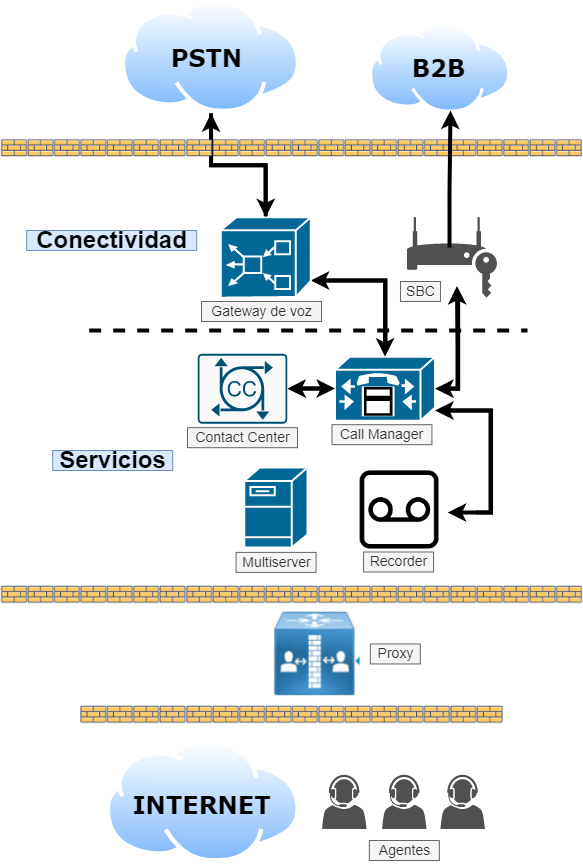
\includegraphics[scale=0.6]{img/fig_arquitectura}
  \caption{Diseño a alto nivel de la arquitectura montada}
  \label{figura:fig_arquitectura}
\end{figure}

\section{Diagrama de flujo}
\label{sec:flujo}

En el siguiente diagrama, se muestra el flujo básico que siguen los dos tipos posibles de llamadas (tanto salientes como entrantes):
\begin{enumerate}
  \item Un \textbf{\textcolor{red}{cliente externo}} hace una llamada al número de atención telefónica. El proveedor enruta la llamada al gateway, que la redirige al Call Manager. Desde el Call Manager se enruta la llamada a través de un puerto virtual específico al Contact Center, el cual consulta los agentes disponibles y hace una asignación basada en ciertos criterios de la empresa en conjunto con las opciones marcadas por el cliente en la locución de bienvenida si la hubiese (IVR o \emph{Interactive Voice Response}).
  
  En el instante en el que un agente descuelga la llamada, el cliente software del agente \textbf{\textcolor{blue}{envía a la grabadora}} todo el tráfico RTP que se ha generado punto a punto, tanto el de origen suyo como el de origen del llamante externo, a través del SIP trunk que sale del Call Manager.
  
  En caso de sentido contrario de llamada el agente marcará la numeración telefónica de un cliente externo, lo que provocará que el call manager enrute la llamada al gateway y éste la saque por el acceso primario al proveedor. En este momento, el proveedor consultará sus tablas de numeración y enlazará la llamada con el destino.
  \item Un \textbf{\textcolor{green}{trabajador de una empresa}} a la que da soporte esta solución llama al servicio técnico. El Call Manager de esa misma empresa enruta la llamada hacia el extremo de su red, a través del cual se conecta con nuestro elemento de borde, el SBC. Dicho SBC enruta la llamada por medio de un SIP Trunk hacia nuestro Call Manager. En este momento, suceden los mismos flujos que en la anterior casuística:
  \begin{itemize}
    \item Asignación de agente mediante Contact Center y establecimiento de sesión punto a punto.
    \item Grabación de llamada \textbf{\textcolor{blue}{a través de la grabadora}} al comienzo de la conversación mediante el envío del flujo RTP por parte del cliente software del agente.
  \end{itemize}
  En caso de sentido contrario de llamada el agente marcará la numeración telefónica del trabajador, lo que provocará que el call manager enrute la llamada al SBC y éste conecte con el Call Manager de la otra empresa. A partir de ahí el flujo es opaco a nosotros, pero es de suponer que la lógica será parecida a la nuestra.
\end{enumerate}

\begin{figure}[!]
  \centering
  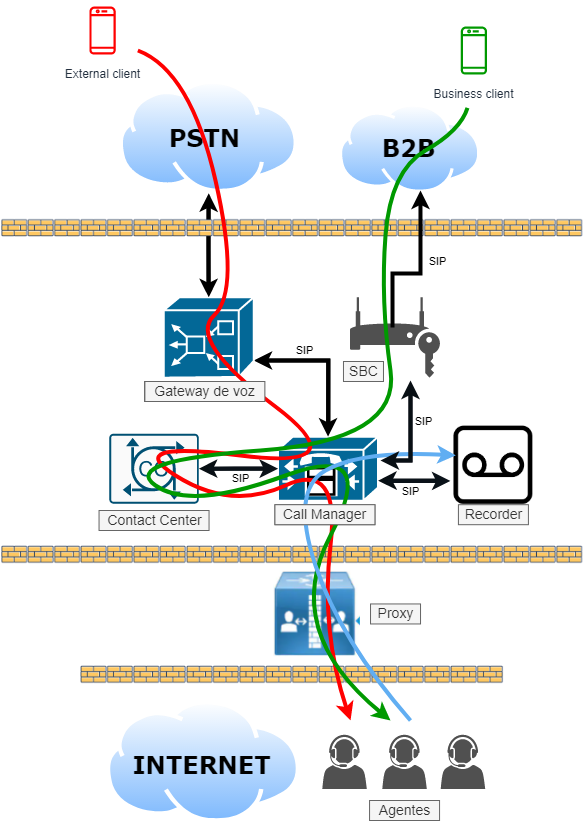
\includegraphics[scale=0.6]{img/fig_callflow}
  \caption{Diagrama de flujo SIP general}
  \label{figura:fig_callflow}
\end{figure}

\section{Configuración de los componentes}
\label{sec:config}

\subsection{Virtualización}
\label{sec:vmware}
Los servidores físicos se configuraron inicialmente con los ajustes de red básicos, que son la IP, la máscara de subred y el gateway. Sobre esta capa de configuracion, está instalado el aplicativo de virtualización llamado VMWare. 

VMWare es una solución basada en el acceso a un escritorio remoto que permite a los usuarios ejecutar máquinas virtuales. Se trata de un sistema que permite operar con software, emulando a un sistema físico (un computador, un hardware, etc.). Esta plataforma permite dividir un único servidor físico en múltiples máquinas virtuales.

Se utilizan funciones especiales en CPU x86 de 64 bits modernas para crear máquinas virtuales seguras y completamente aisladas que encapsulan un sistema operativo y sus aplicaciones. La capa de virtualización de VMware asigna los recursos de hardware físicos a los recursos virtuales de la máquina virtual, por lo que cada máquina virtual cuenta con una CPU, una memoria, unos discos y unos dispositivos de E/S propios, y equivale en su totalidad a una máquina x86 convencional. VMware Workstation, que es el hipervisor de escritorio, se ha instalado en el sistema operativo host. Con ello se consigue una amplia compatibilidad de hardware al heredar del host la conciliación con los dispositivos.

En la Figura ~\ref{figura:fig_vmware} se presenta el aspecto de la interfaz del aplicativo con varias de las máquinas virtuales instaladas y parte de la información sensible ocultada.

\begin{figure}[h!]
  \centering
  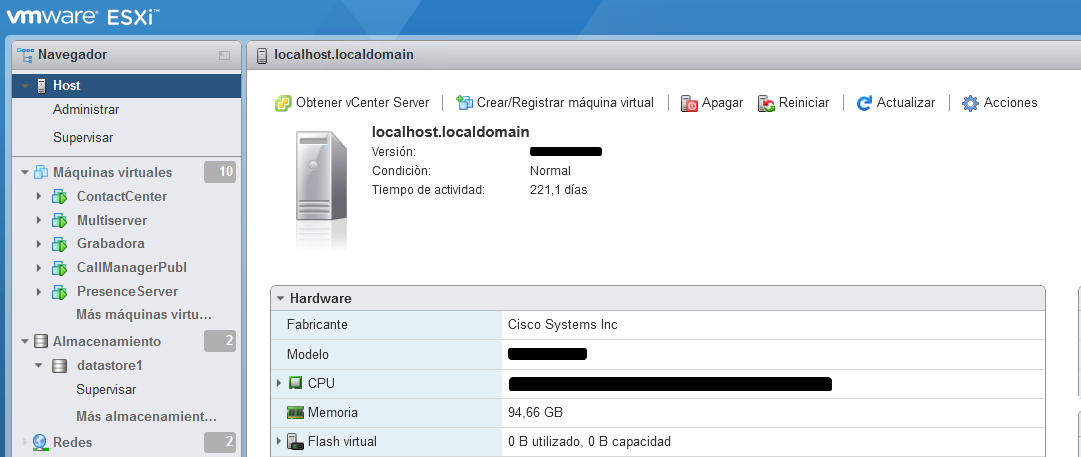
\includegraphics[scale=0.8]{img/fig_vmware}
  \caption{Interfaz web de VMWare}
  \label{figura:fig_vmware}
\end{figure}

\subsection{Multiserver}
\label{sec:multiserver}
Hay varias gestiones y configuraciones necesarias para complementar la solución que no se pueden hacer únicamente desde los equipos de Cisco, por lo que hubo que instalar servidores Windows y CentOS para llevarlas a cabo. Dichos servidores están representados en el esquema general de la arquitectura como el Multiserver.

Servicios que han sido desplegados:
\begin{itemize}
  \item \textbf{DNS}. Para el despliegue de este servicio se ha optado por Windows Server. Dicho SO dispone de una herramienta llamada Server Manager, que permite la instalación y configuración de un DNS propio de Microsoft (Figura ~\ref{figura:fig_dns}). Tras seguir los pasos y finalizar la instalación, se procedieron a crear las zonas de búsqueda y los registros con los nombres que se asociaron a cada máquina virtual, también llamados FQDN (Fully Qualified Domain Name). A través de esos nombres se podrá acceder a la interfaz de gestión web de las máquinas que lo tengan habilitado. Por ejemplo, si al Call Manager se le ha asociado la FQDN ``vmcucm'' (Figura ~\ref{figura:fig_dominios}), el acceso a la gestión web de esa máquina será https://vmcucm.dominio.es. Aunque en este caso fue instalado y configurado de cero, es habitual que el DNS lo proporcione la empresa en la que se hace la instalación.
  
  También se ha instalado en este sistema una base de datos Microsoft SQL Server, que se explicará más adelante cuál es su utilidad.

  \item \textbf{Certificate Authority (CA)}. Una Autoridad de Certificación es una entidad de confianza, responsable de emitir y revocar los certificados digitales. Un certificado es un archivo que contiene el nombre del titular del certificado, la clave pública y la firma digital de la autoridad certificadora que emite el certificado, que prueba la identidad del propietario del certificado. 
  Mediante dichos documentos, los distintos elementos de la solución confiarán entre ellos al validar sus identidades y la comunicación será segura.
  Esta CA se ha configurado en un SO CentOS, que es una distribucion de Linux de código abierto.
  Este elemento se ha desplegado con unas especificaciones poco exigentes pero con bastante almacenamiento pues su obejtivo será, ademas de actuar de entidad certificadora, el de almacenar los datos de los chats persistentes y las imágenes que los agentes se envíen entre sí.

  \item \textbf{Cliente Windows}. Como el entorno no tiene conexión con el exterior, se necesita una herramienta para el análisis y \emph{troubleshooting}. Para ello se ha instalado una máquina virtual con Windows 10, que dispone también de un cliente de jabber y software adicional para el análisis del tráfico SIP. De esa manera se pueden hacer llamadas de prueba de forma interna, capturar paquetes o instalar herramientas de Cisco como el Real Time Monitoring Tool (RTMT), que sirve para ver y exportar los logs del Call Manager y Contact Center.
\end{itemize}

\begin{figure}
  \centering
  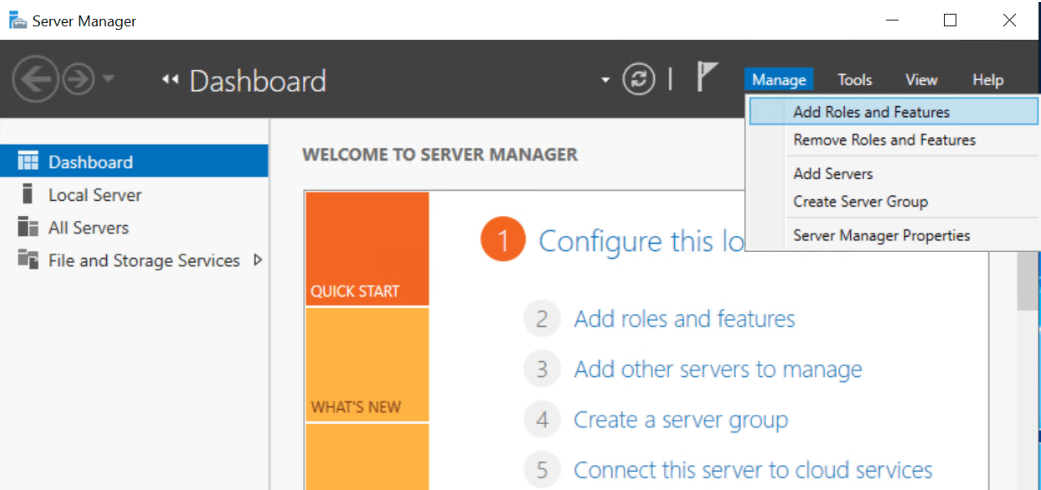
\includegraphics[scale=0.85]{img/fig_dns}
  \caption{Creación de DNS en Server Manager}
  \label{figura:fig_dns}
\end{figure}

\begin{figure}
  \centering
  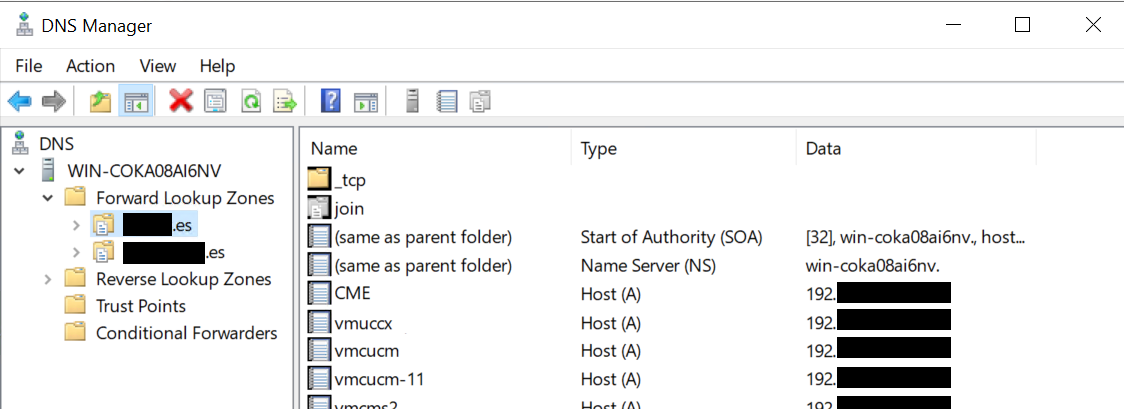
\includegraphics[scale=0.8]{img/fig_dominios}
  \caption{Ejemplo de registros en el DNS}
  \label{figura:fig_dominios}
\end{figure}

\subsection{Grabadora}
\label{sec:grabadora}
Se ha instalado un software de terceros que se integra con la solución de colaboración de Cisco, y que tiene acceso vía web. El panel de la grabadora proporciona una descripción completa de las llamadas por día, la duración promedio de las llamadas, las llamadas activas actuales, etc. Dicha interfaz almacena estadísticas muy detalladas (figuras ~\ref{figura:fig_portada_recorder}, ~\ref{figura:fig_grabaciones} y ~\ref{figura:fig_grabaciones_02}) que pueden ser utilizadas para una exportación con criterios de búsqueda muy ajustados.

Por ejemplo, en la figura ~\ref{figura:fig_filtros} está programada una búsqueda que aúna tres criterios: que las llamadas sean posteriores al 1 de junio de 2022, que superen los 10 minutos de duración y que sean entrantes.
De esa manera, podemos localizar a los agentes que se estén excediendo reinicidentemente del tiempo límite y echarles un rapapolvo.
Estas combinaciones para las búsquedas pueden guardarse con un nombre identificativo y ahorrar mucho tiempo y trabajo en posteriores aplicaciones del mismo filtro.

\begin{figure}[h!]
  \centering
  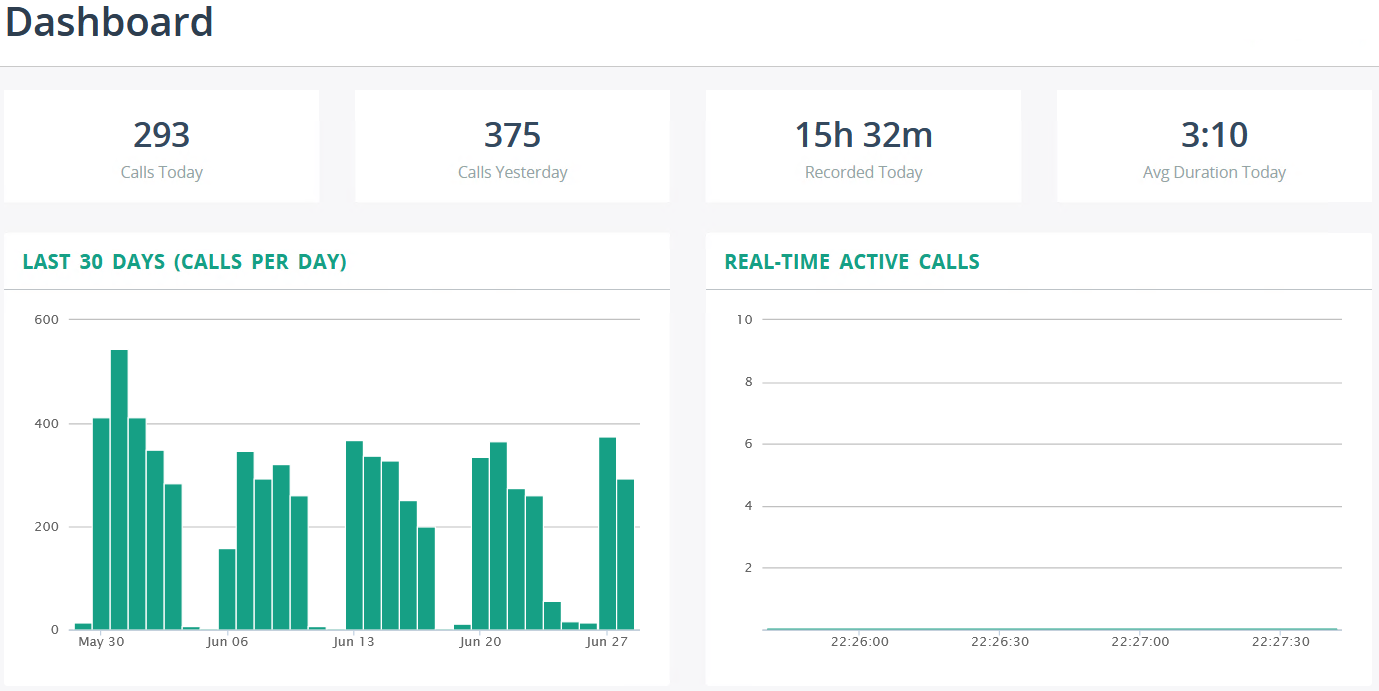
\includegraphics[scale=0.65]{img/fig_portada_recorder}
  \caption{Panel de resumen de la grabadora}
  \label{figura:fig_portada_recorder}
\end{figure}

\subsubsection{Instalación}
\label{sec:instalacion_grabadora}

La instalación se ha realizado mediante una plantilla OVA, que es una máquina virtual preinstalada con sistema operativo definido (CentOS) y el software de grabación de llamadas.
Esta plantilla es la solución ideal para este contexto, ya que su descarga es rápida al encontrarse comprimida y es fácil de importar al entorno de VMWare.
Al no disponer de enlaces de descarga, se ha adquirido mediante petición al fabricante desde su página web.

\subsubsection{Configuración}
\label{sec:configuracion_grabadora}

Se pueden separar las configuraciones realizadas en dos partes:
\begin{enumerate}
  \item Configuraciones en la GUI del software vía web. Desde este lado se han añadido los agentes de forma manual, los grupos a los que pertenece cada uno, los roles, los supervisores, el licenciamiento y los ajustes de almacenamiento y codificación.
  \item Configuraciones del lado del Call Manager. Se ha habilitado un SIP Trunk directo hacia la grabadora, se ha configurado un perfil de seguridad SIP, un perfil SIP, un perfil de grabacion y un patrón de rutas que apunta a la grabadora.
\end{enumerate}

\begin{figure}
  \centering
  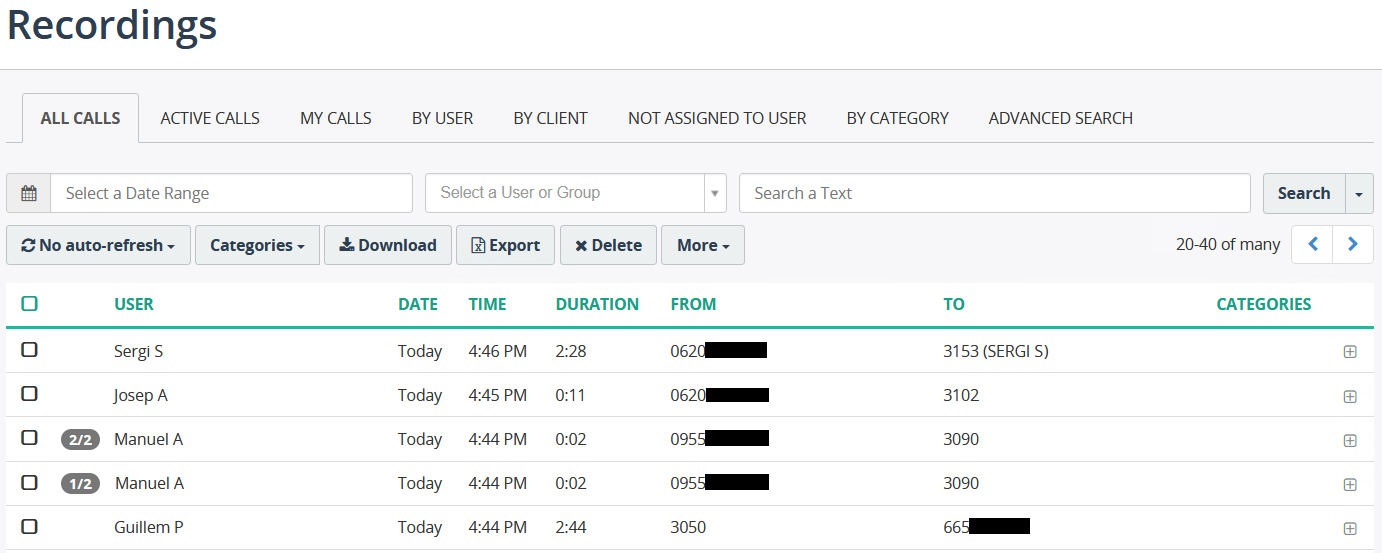
\includegraphics[scale=0.65]{img/fig_grabaciones}
  \caption{Aspecto de la interfaz de visualización de grabaciones}
  \label{figura:fig_grabaciones}
\end{figure}

\begin{figure}
  \centering
  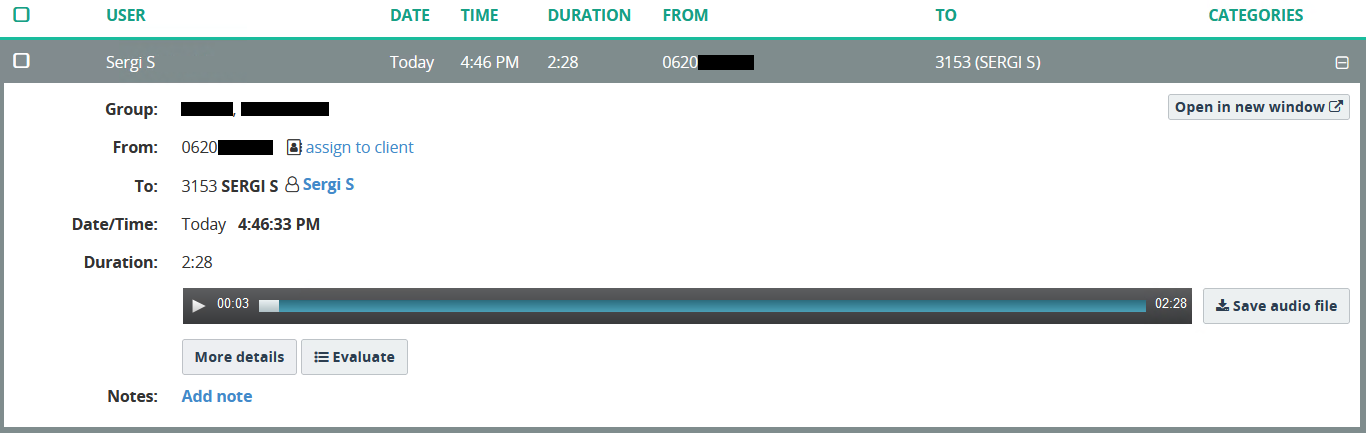
\includegraphics[scale=0.65]{img/fig_grabaciones_02}
  \caption{Detalle de una grabación específica}
  \label{figura:fig_grabaciones_02}
\end{figure}

\begin{figure}
  \centering
  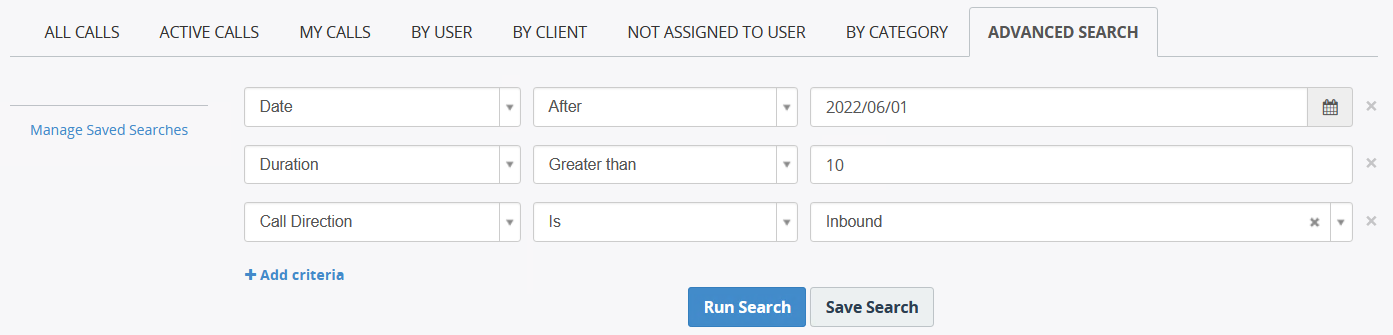
\includegraphics[scale=0.65]{img/fig_filtros}
  \caption{Ejemplo de búsqueda con criterios}
  \label{figura:fig_filtros}
\end{figure}


\subsection{Call Manager}
\label{sec:call_manager}

La solución cuenta con varios Call Manager:
\begin{itemize}
  \item CUCM (Cisco Unified Call Manager). Entre todos los que hay instalados, uno es el que tiene el papel principal y actúa de \emph{master}, también llamado \emph{publisher}. En él se realizarán los cambios, que serán propagados al resto de Call Managers. Además, hay otros dos CUCM más que actúan de \emph{subscriber}, redundando así la solución para tener mayor capacidad de usuarios y llamadas y también ganar robustez frente a caídas de servicio.
  \item CUCM IM\&P (Cisco Unified Call Manager Instant Messaging and Presence), que son los encargados de proveer del servicio de presencia en la aplicación de mensajería (offline, online, ausente...) mediante el protocolo XMPP (\emph{Extensible Messaging and Presence Protocol}). También existen varios para redundancia, aunque al tratarse de una versión alternativa de Call Manager, ambos actúan como \emph{subscribers}.
  Es en estos elementos donde se habilita la mensajería instantánea entre agentes de la organización mediante el aplicativo Jabber. Para añadir la característica de chat persistente (que se mantenga entre sesiones), se ha integrado la base de datos SQL Server que se desplegó en el servidor de Windows y también se ha configurado una ruta de la máquina con CentOS para el almacenamiento de imágenes, texto y metadatos.
\end{itemize}

\subsubsection{Configuraciones}
\label{sec:conf_cucm}
En el Call Manager \emph{publisher} se han realizado los ajustes más importantes y esenciales para el funcionamiento del entorno. A continuación se enumeran los más importantes y su propósito:
\begin{enumerate}
  \item Activación de servicios, tales como el DHCP (\emph{Dynamic Host Configuration Protocol}) que provee de IP automáticamente a los agentes que se registran o el TFTP (\emph{Trivial File Transfer Protocol}) que provee de la última actualización de software a los dispositivos de cisco, entre otros muchos servicios.
  \item \emph{Device Pools}, que establecen un orden de prioridad entre todos los Call Manager de la solución sobre los que se registrarán los agentes. De esta manera se balancea la carga de usuarios y se podrá liberar opcionalmente el publisher de capacidad de procesamiento, ya que será el que se ocupará de alojar los servicios más importantes.
  \item Particiones y \emph{Calling Search Spaces}, que identifican cada agente en un grupo determinado con una serie de privilegios de llamada concretos.
  \item \emph{Route Patterns}, que consisten en una cadena de dígitos y un conjunto de manipulaciones de dígitos que enrutan llamadas a un SIP Trunk. Estos patrones son muy útiles, pues brindan una gran flexibilidad en el diseño de la red. Además, trabajan en conjunto con filtros de ruta y listas de rutas para dirigir llamadas a dispositivos específicos y para incluir, excluir o modificar patrones de dígitos.
  \item Extensiones, que serán el número de teléfono interno de cada agente. Cada extensión estará asociada a un dispositivo, que será el PC con el que se conecte cada uno desde su localización. Cada dispositivo configurado consume una licencia de Call Manager, por lo que habrá tantas como agentes hubiera, teniendo en cuenta que cada uno utilizará únicamente su PC como dispositivo de registro.
  \item \emph{Music on Hold} y \emph{announcements}, que serán las locuciones de bienvenida y la música que se reproduzca cuando el llamante quede en espera a que un agente descuelgue.
  \item \emph{CTI Route Point} (Computer Telephony Integration), que son los \emph{triggers} que enlazan una llamada entrante a un agente libre mediante un \emph{CTI port}. Se trata de una numeración corta resultado de una transformación de una numeración real (número de atención al cliente). Este \emph{CTI Route Point} está asociado a unos puertos CTI virtuales, a través de los cuales se enlaza la llamada con un agente.
  \item \emph{SIP Trunk} o troncal SIP, es una conexión virtual a través de internet que se crea entre dos elementos para el tráfico de voz, principalmente. Se ha creado uno hacia cada elemento que tiene un rol en el tráfico de voz, es decir: los gateways, SBCs, el CUCM IM\&P y la grabadora. En resumidas cuentas, a estos enlaces se les asocia una IP de destino y un perfil SIP, junto a otros aspectos como el método de entrega de DTMF (\emph{Dial Tone Multi Frecuency})\footnote{Tono que se genera al pulsar las teclas de marcado.} en RFC 2833. Esta especificación de entrega de DTMF~\cite{rfc2833} establece un formato de payload de RTP para el soporte de marcación de dígitos, en este caso la marcacion a la que invitan las locuciones de bienvenida.
  \item Usuarios, que tendrán especificados el nombre y apellidos y las credenciales para loguearse a la plataforma. También tienen un dispositivo vinculado creado anteriormente, junto a dos extensiones: la interna y la IPCC, que será la asociada al Contact Center.
\end{enumerate}

Cisco mediante Call Manager permite una gestión de los perfiles de usuario \emph{end-point} y de los derechos basados en éstos para diversos grupos, departamentos y divisiones, gestionados por usuarios administradores.

\subsection{Contact Center}
\label{sec:contact_center}

El objetivo del Contact Center es manejar unos puertos virtuales que estarán permanentemente en escucha esperando que se reciba una llamada entrante y asociarla a un agente que esté disponible en ese momento, respentando pausas de unos segundos entre cada llamada (la cantidad de segundos de pausa se ha definido en base a preferencias de la empresa).

Cada agente dispone de un usuario con unas características y \emph{skills} o habilidades definidas. Se les puede asignar un conocimiento, como por ejemplo inglés, y un nivel de experiencia en ese conocimiento, de manera que sirva de medida para encontrar el agente más adecuado a cada circunstancia.
Al ser un servicio compartido con agentes en nómina de la empresa en la que se ha montado esta solución, muchas habilidades tendrán que ver con conocimientos concretos de varias empresas. Por ejemplo puede haber un agente que tenga habilidades de  información comercial de Heineken, postventa de Balay, información de producto de Telefónica, alemán\ldots

Todos y cada uno de los clientes contratantes de este servicio tiene un número de atención telefónico asignado, el cual será transformado a la entrada del Call Manager a una numeración más corta de 4 dígitos llamada \emph{CTI Route Point} mediante las reglas establecidas en los \emph{Translation Patterns}. Esta numeración, también llamada \emph{trigger}, está asociada a una cantidad de puertos que se definen cuando se crea dicho \emph{trigger} (figura ~\ref{figura:fig_ctiports}). El número de puertos CTI virtuales de los que disponga este \emph{trigger} será el número máximo de llamadas paralelas que puede atender este cliente, por lo que cuanto mejor servicio contrate, más puertos simultáneos podrá disponer. 

Es común que cada cliente puede disponer de varios \emph{triggers} orientados cada uno a un departamento en concreto, por ejemplo un \emph{trigger} dirigido a consultas de problemas informáticos, otro dirigido a consultas de postventa\ldots

\begin{figure}
  \centering
  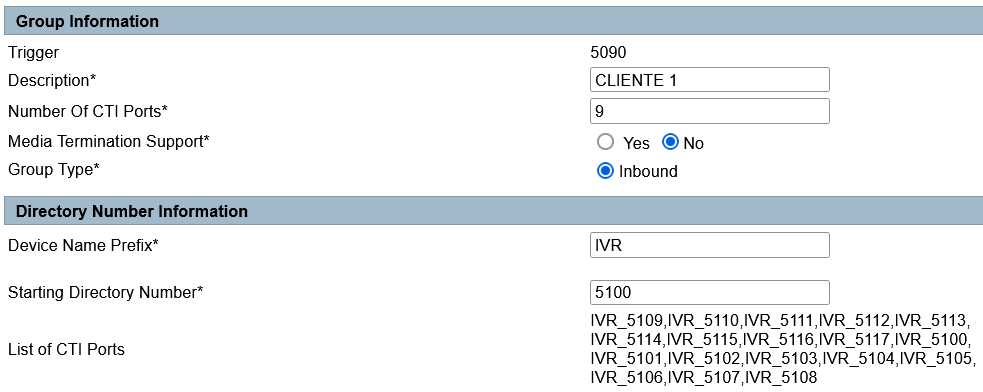
\includegraphics[scale = 0.85]{img/fig_ctiports}
  \caption{Puertos asignados a un \emph{trigger}}
  \label{figura:fig_ctiports}
\end{figure}

\begin{figure}
  \centering
  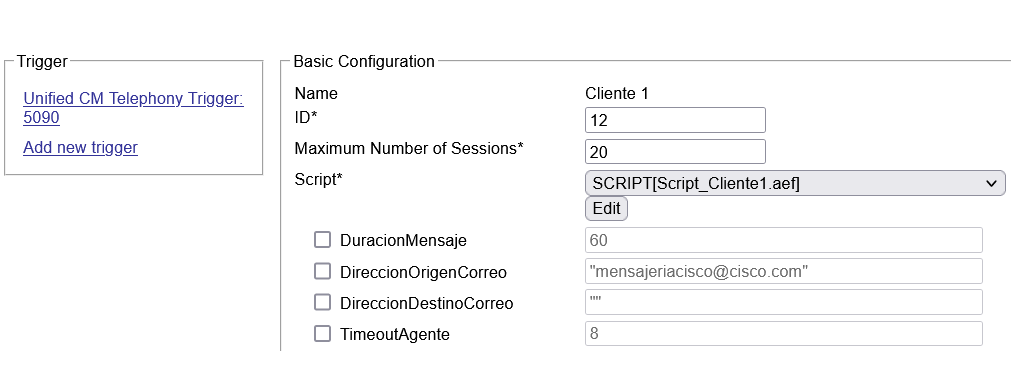
\includegraphics[scale = 0.85]{img/fig_aplicacion}
  \caption{Aplicación asociada a un \emph{trigger}}
  \label{figura:fig_aplicacion}
\end{figure}

El \emph{trigger} está enlazado a una aplicación (figura ~\ref{figura:fig_aplicacion}), la cual define un script que se ejecutará para todos los puertos de este \emph{trigger}. Este script es el encargado, entre otra cosas, de:
\begin{itemize}
  \item Reproducir la locución de bienvenida.
  \item Lanzar las opciones de marcado de dígito
  \item En base a los dígitos marcados, buscar un agente que satisfaga los requisitos de habilidades y expertise.
  \item De los agentes  filtrados, buscar el que esté disponible.
  \item Asignar la llamada.
  \item Recoger estadísticas.
\end{itemize}


En el ejemplo de la figura ~\ref{figura:fig_script} se puede ver una sección del script de un cliente en el que la llamada entra a la cola, se reproduce una locución que anuncia el comienzo de la cola y entonces comienza la lógica de búsqueda (función ``SelecciónRecursosCAU'', definida en otra sección del script) y asignación de agente.

\begin{figure}[h!]
  \centering
  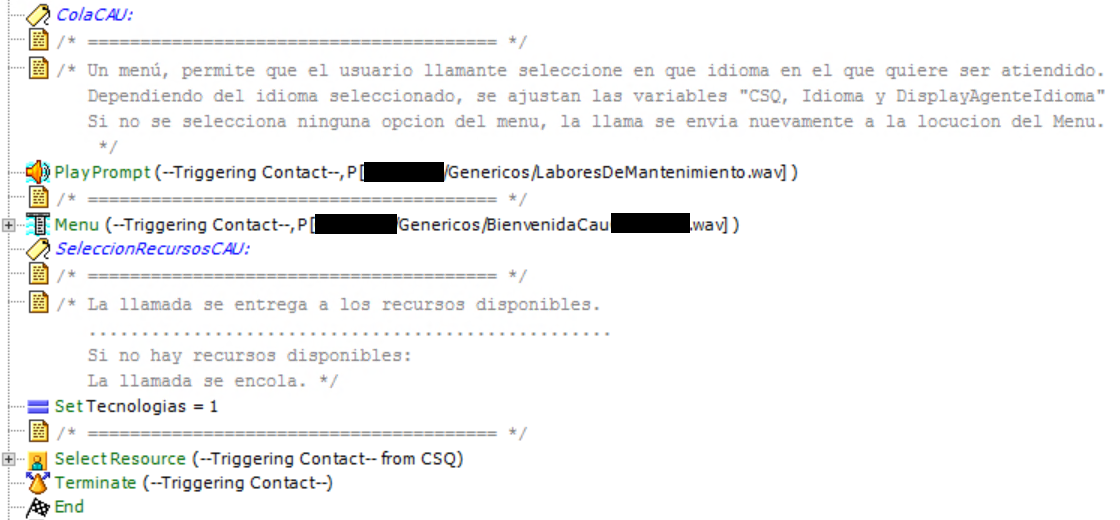
\includegraphics[scale = 0.8]{img/fig_script}
  \caption{Sección real de un script de asignación de recursos}
  \label{figura:fig_script}
\end{figure}

Las posibilidades de estos scripts son muy extensas, llegando a poder, en el caso de uno de los clientes, asignar una extensión que conecte con el Contact Center e iniciar la grabación de un mensaje de voz para colocarlo automáticamente al inicio o al final de la locución de bienvenida con el objetivo de dar aviso de una incidencia masiva en el servicio. 
Estas grabaciones pueden ser restringidas mediante el marcado de una contraseña, de modo que sólo los administradores puedan ejecutarlas.

Aunque en este caso se han configurado en español, todas las locuciones se pueden cambiar de idioma si se desea, pues son lecturas de texto ejecutadas por sintetizadores de voz.

\subsection{Gateway}
\label{sec:gateway}

El proveedor de telefonía ha provisto de un enlace Primario o E1 con un ancho de banda total de 2048Kbps, que consta de 32 canales E0 a 64Kbps, debido a la codificación G.711~\cite{itu}. De esos 32 canales, 2 son para señalizacion y 30 están destinados a datos. 
Esta velocidad de 64K parte del criterio de Nyquist, en donde se formula que para recuperar de forma digital una señal analógica y muestrearla correctamente debemos hacerlo a una tasa dos veces superior al ancho de banda. 
Con un ancho de banda de la señal analógica de 4KHz se debe muestrear a 8KHz, que usando 8 bits por muestra da el resultado de 64Kbps.

La frecuencia máxima (banda en frecuencia limitada) en una señal analógica $x_{a}(t)$ podemos denominarla como $F_{max}$  o $B$. Si la señal se muestrea a una tasa mínima del doble de esa frencuencia, entonces $F_{s} \geq 2B$.

Para la multiplexación de la señal, la técnica más utilizada en la actualidad, especialmente en la transmision de sistemas digitales, es la multiplexación por división de tiempo (TDM en inglés). Mediante esta técnica, se asignan ranuras o \emph{slots} de tiempo a cada trama de las señales originarias (figura ~\ref{figura:fig_tdm}). Este tipo de asignación fija no es la mejor forma de aprovechar el espectro disponible, ya que si un señal no está enviando datos durante un tiempo determiando (silencio), se están desperdiciando ranuras. Sin embargo, este inconveniente no sucede en el mundo digital, donde el total del ancho de banda se reasigna de forma dinámica en los recursos que lo necesiten.

\begin{figure}
  \centering
  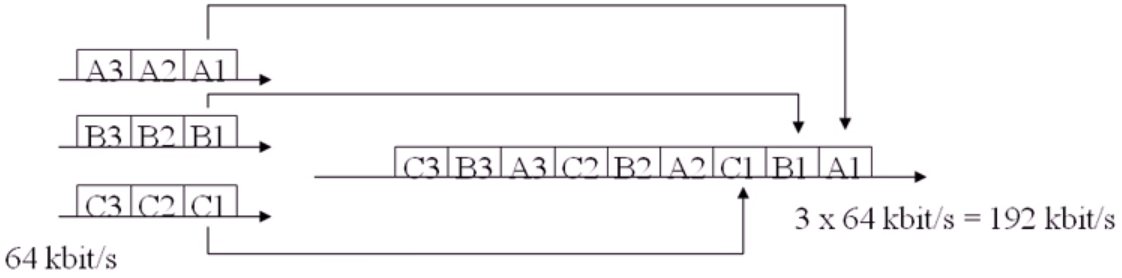
\includegraphics[scale=0.7]{img/fig_tdm}
  \caption{Ejemplo de multiplexación TDM}
  \label{figura:fig_tdm}
\end{figure}

En este contexto, el Gateway de voz es un elemento imprescindible para el funcionamiento de un sistema de Voz IP con conexión a la red pública, pues es el responsable de hacer la traducción entre el mundo interno digital y el externo analógico a través de sus puertos FXO (\emph{Foreign eXchange Office}). Su trabajo es convertir la señal analógica multiplexada en TDM, a una paquetización para el envío a través de una red IP. De forma análoga, un gateway también realiza el proceso contrario: convierte los paquetes digitales a tráfico TDM para transportarlos a través de la PSTN.

Para esta labor, la reconstrucción de la señal analógica es matemáticamente posible a partir de las muestras de la señal digital. Se realiza un sumatorio de todas las muestras y, mediante una función de interpotalción que define la naturaleza del sistema interpolado, se obtiene la siguiente ecuación:

\large
\[
  x_{a}(t) = \sum_{n=\infty}^\infty x_{(n)}i(t-nt_{s})
\]
\\
\normalsize
Donde $x_{(n)}$ es la función discreta, e $i(t-nt_{s})$ es la funcion de interpolación que define el desfase de cada impulso.

Existen dos gateways redundados geográficamente, los cuales disponen de una conexión E1 independiente contra el proveedor telefónico. En el momento en el que se realiza una llamada entrante al sistema, el proveedor posee dos alternativas para la entrega de la llamada a los gateways:

\begin{enumerate}
  \item \textbf{Activo/Activo}, configuración que envía las llamadas por ambos gateways simultáneamente. Bajo ciertos criterios de decisión, como por ejemplo la carga de llamadas en cada localización o la congestión existente en el par de cobre, el proveedor decidirá balancear las llamadas y entregarlas a uno u otro.
  \item \textbf{Activo/Pasivo}, lógica que entrega las llamadas siempre al mismo gateway. En el momento en que haya una caída y no responda, su sistema de \emph{health check} descubrirá que la conexión con el primer gateway está caída, por lo que comenzará a enrutar las llamadas hacia el segundo. Este cambio de enrutamiento debería llevarse a cabo idealmente en apenas unos segundos.
\end{enumerate}

En el caso que mencionaba al inicio de este subcapítulo, hablaba del uso de G.711 en los canales previos a la multiplexación, pues es uno de los estándares de la ITU-T más usados en telefonía. Sin embargo, cada red privada tiene a su disposición la elección de códec destinado a sus comunicaciones internas, lo que puede provocar disconformidad a la hora de enrutar llamadas al exterior o a otras redes privadas. 
Para solventar este inconveniente, el gateway es capaz también de realizar una transcodificación de la señal entrante y adaptarla al medio de destino, de manera que ambos extremos hablen el mismo ``idioma''. Dicha transcodificación no ha sido necesaria entre nuestra red privada y la PSTN al utilizar ambos la misma codificación, sin embargo si ha sido imperativa su implementación para la comunicación con los entornos de las otras empresas separadas por el SBC, aunque es éste el que se encarga en este caso de realizar dichas transcodificaciones.

\subsection{Session Border Controller}
\label{sec:sbc}

La seguridad de los entornos empresariales es un factor indispensable a la hora de planear una arquitectura que abra sus puertas a conexiones externas, es por ello que los firewalls son elementos necesarios en estas soluciones. Sin embargo, su operatividad está basada en NAT, algo incompatible con el tráfico VoIP.
Para solventarlo, se ha implementado un elemento llamado SBC, que toma parte activa y actúa de firewall de voz, impidiendo conexiones ilícitas y bloqueando intrusiones. Este elemento está conectado directamente contra el Call Manager, transcodificando también las llamadas al códec que se usa en el Call Manager destino (figura ~\ref{figura:fig_sbc}). Cada enlace a los clientes de esta empresa está definido mediante un SIP Trunk, que dispone de su propio puerto físico en el SBC.

\begin{figure}[h]
  \centering
  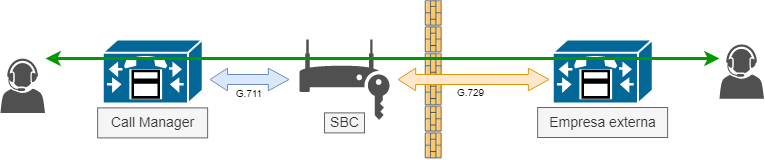
\includegraphics[scale=0.55]{img/fig_sbc}
  \caption{Flujo de llamadas a través de un SBC}
  \label{figura:fig_sbc}
\end{figure}

Cuando una llamada entrante desde el Call Manager posee un patrón en el número marcado, si este patrón hace match con uno registrado en el SBC, es entonces cuando se enruta la llamada por el puerto correspondiente hacia su destino.
Por ejemplo, si un agente de la empresa marca la extensión de un usuario de un cliente precedida por un patrón numérico, ese patrón es detectado por las políticas de enrutado configuradas en el Call Manager, que enviará la llamada al SBC. El SBC comparará el patrón con su tabla de destinos, y con el que coincida la numeración es con quien creará el enlace.

Además de las funciones ya mencionadas, otra muy interesante y que está siendo de mucha utilidad es la posibilidad de manipulación de mensajes. Se puede analizar la cabecera de una petición http y adaptar los parámetros de nuestro interés. Entre otras manipulaciones, se ha aplicado una que modifica la cantidad de reenvíos máximos permitidos de la petición:

\begin{verbatim}
MATCH
Message Type: any		
Condition:	header.request-uri.methodtype == '8'

ACTION
Action Subject:	header.max-forwards.val	
Action Type:	Modify	
Action Value:	'10'
\end{verbatim}

Por último, tras una configuración completa del SBC primario, se procedió a instalar un segundo en otro CPD de manera que, al igual que el resto de elementos de la solución, diponga de redundancia. Sin embargo, este tipo de redundancia es un poco especial, pues se ha configurado de tal manera que si se cae el servicio en alguno de los dos SBC las llamadas en curso no se cortarán, sino que sufrirán un silencio de pocos segundos y se reestablecerá la conexión, conduciendo el flujo de la llamada por el segundo SBC. Este tipo de redundancia se denomina \emph{High Availability} (HA) o Alta Disponibildiad en castellano.

La Alta Disponibilidad se diferencia de la redundancia básica porque ofrece un servicio de sustitución casi inmediato, impidiendo que se produzca un corte en el servicio aunque sea de pocos minutos. En esta configuración, ambos SBC comparten la misma IP, testigo que se turnan estos sistemas cuando uno de ellos está caído. Así, las llamadas de los elementos externos no tienen que cambiar de destino, ya que realmente la IP no ha cambiado sino que ha tomado el relevo el elemento funcional de los dos.

\subsection{Monitorización}
\label{sec:monitoring}

Muchas organizaciones necesitan llevar un control en directo de sus sistemas para comprobar que funcionan correctamente y con el objetivo de conseguir una conexión permanente y sin caídas. Es el caso de la empresa en la que se ha implementado este proyecto, pues es primordial que el servicio que ofrece se vea afectado lo mínimo posible por imprevistos. Mediante protocolo SNMP (\emph{Simple Network Management Protocol}), un administrador red es capaz de realizar un \emph{health check} y consultar o modificar ciertos servicios de cada máquina del entorno. Para ello, se configura una cadena de caracteres llamada \emph{Community String}, compatible con versiones de SNMPv1 y SNMPv2.

Cuando se envía la \emph{Community String} correcta al dispositivo de la red, el dispositivo devuelve un conjunto de datos depurados al administrador. Se puede configurar una cadena pública, que actúa como una solicitud de "solo lectura", lo que permite que el administrador consulte, pero no modifique, el dispositivo remoto; o una cadena privada, que es una opción más potente que permite al administrador leer y escribir en el sistema remoto.

Para llevar a cabo las consultas SNMP se pueden emplear varios programas de terceros como Solar Wind o Spectrum. En la figura ~\ref{figura:fig_spectrum} se muestra como se ha implementado esta monitorización con Spectrum.
\begin{figure}
  \centering
  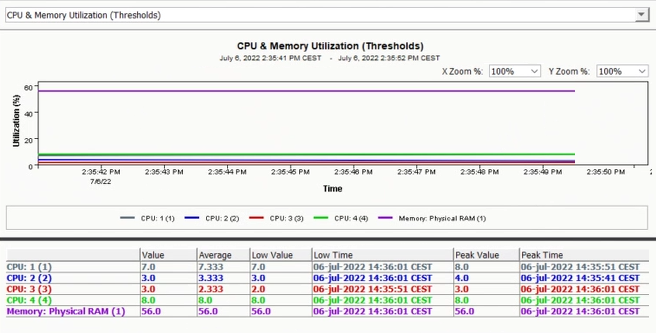
\includegraphics[scale = 1.2]{img/fig_spectrum}
  \caption{Monitorización de CPUs y RAM del CUCM \emph{publisher}.}
  \label{figura:fig_spectrum}
\end{figure}



%%%%%%%%%%%%%%%%%%%%%%%%%%%%%%%%%%%%%%%%%%%%%%%%%%%%%%%%%%%%%%%%%%%%%%%%%%%%%%%%
%%%%%%%%%%%%%%%%%%%%%%%%%%%%%%%%%%%%%%%%%%%%%%%%%%%%%%%%%%%%%%%%%%%%%%%%%%%%%%%%
% EXPERIMENTOS Y VALIDACIÓN %
%%%%%%%%%%%%%%%%%%%%%%%%%%%%%%%%%%%%%%%%%%%%%%%%%%%%%%%%%%%%%%%%%%%%%%%%%%%%%%%%

\cleardoublepage
\chapter{Experimentos y validación}

He realizado una captura de una llamada que he hecho desde mi teléfono móvil hasta el teléfono de atención al cliente de uno de los clientes de la empresa que aloja la solución. El flujo de datos atravesaría en orden los siguientes elementos:
\begin{enumerate}
  \item Llamada desde mi móvil perticular por la PST al número de atención al cliente.
  \item Llegada al Gateway. El gateway lo enruta al interior.
  \item Llegada al Call Manager.
  \item Call Manager comienza flujos de procesos paralelos con el Contact Center y con la grabadora.
  \item El flujo de voz continúa hacia el proxy.
  \item El proxy enlaza la llamada con los agentes a través de la red de Internet.
\end{enumerate}

\begin{figure}
  \centering
  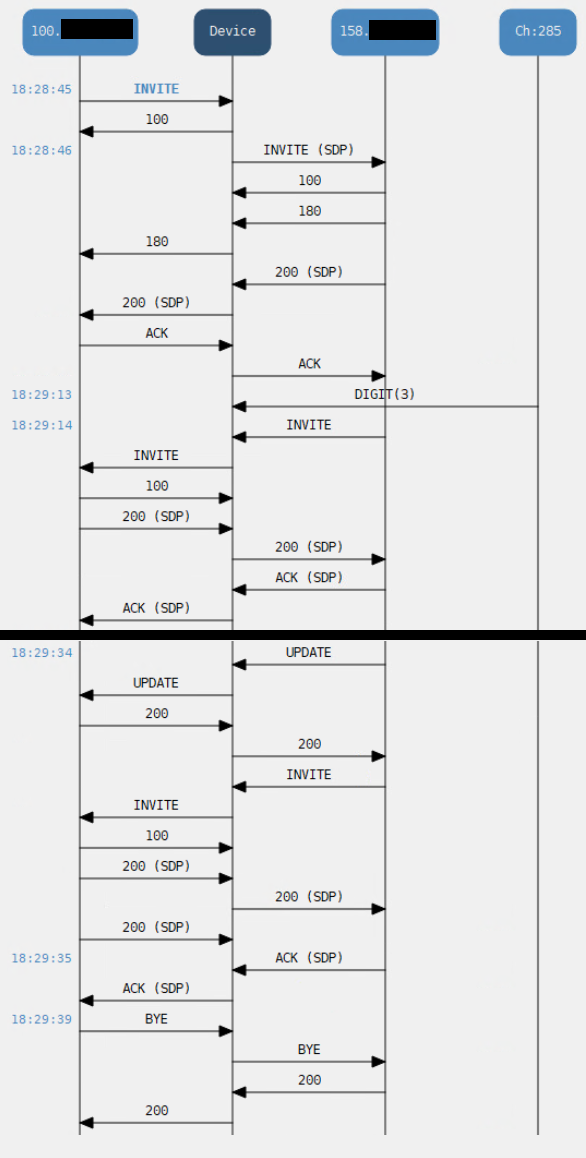
\includegraphics[scale = 1.1]{img/fig_sipflow_diagram}
  \caption{Diagrama de flujo en llamada de test}
  \label{figura:fig_sipflow_diagram}
\end{figure}

Una vez analizado el trayecto por el que circula la señal, vamos a ver a más bajo nivel los detalles del flujo SIP. Tomando como referencia la figura ~\ref{figura:fig_sipflow_diagram}, el proceso que sigue la llamada real sería el siguiente:
\begin{enumerate}
  \item Marcado del número de destino. La IP de origen en el gráfico (izquierda) pertenece al gateway, que recibe la llamada externa del teléfono móvil a través de la PSTN, y la está enrutando hacia el interior del entorno a un puerto CTI libre del Call Manager. Se envía una petición INVITE al Call Manager.
  \item El Call Manager reproduce la locución IVR asociada a ese puerto, y el Contact Center lanza el script para la asignación de agente. Pulso el dígito 3 cuando la locución lo indica, y mediante RFC2833 se envía un dígito con payload type 99, de manera que la respuesta se guarda y se utiliza para asignarme el agente idóneo.
  \item Comienzan una serie de reenvíos de petición INVITE mientras la llamada se encuentra en espera, momento en el que suena la música de espera configurada, hasta que el Call Manager envía una actualización de parámetros mediante UPDATE. 
  \item Un segundo después, el Call Manager envía una petición ACK, indicando que se va a establecer la llamada. Comienza el tráfico RTP, en el que un agente humano contesta al teléfono. 
  \item Cuelgo a los 5 segundos alegando una confusión y se envía una petición BYE, que es respondida por un 200OK y se cierra la conexión.
\end{enumerate}
Durante todo este proceso se han ido negociando parámetros distintos dependiendo del tipo de petición. Tenemos como ejemplo la petición invite en la figura ~\ref{figura:fig_sipflow_param1}. Los elementos tapados en Azul corresponden a la IP (gateway) y teléfono del llamante, mientras que los datos tapados en negro corresponden a la IP y teléfono del llamado. Se puede observar:
\begin{itemize}
  \item En la cabecera ``Via'' indica el método y la IP:puerto de origen
  \item En la cabecera ``From'' se indica el teléfono de origen de la llamada y la IP del gateway que la convierte en digital.
  \item En la cabecera ``To'' se define el teléfono y la IP de destino.
  \item En las siguients cabeceras se inidican la fecha, número identificativo de la llamada, métodos permitidos, expiración, número máximo de reenvíos y el tipo y longitud del contenido (SDP).
  \item Comienzan los descriptores SDP, como la versión del protocolo, el creador de la sesión, nombre del medio y dirección de transporte\ldots. Por último las líneas de atributos de la sesión, en la que se describen los distintos atributos que afectan a la media añadiendo información sobre los flujos.
\end{itemize}
En la grabadora también se procesó correctamente la llamada, como muestra la figura ~\ref{figura:fig_grab_test}. Me atendió el agente Abel S, con número de extensión de Contact Center 3104. Si me asignara mi número de teléfono particular como cliente en la opción del apartado ``To'' y volviera a llamar, me identificaría como un usario recurrente que ya ha llamado en ocasiones anteriores.

\begin{figure}
  \centering
  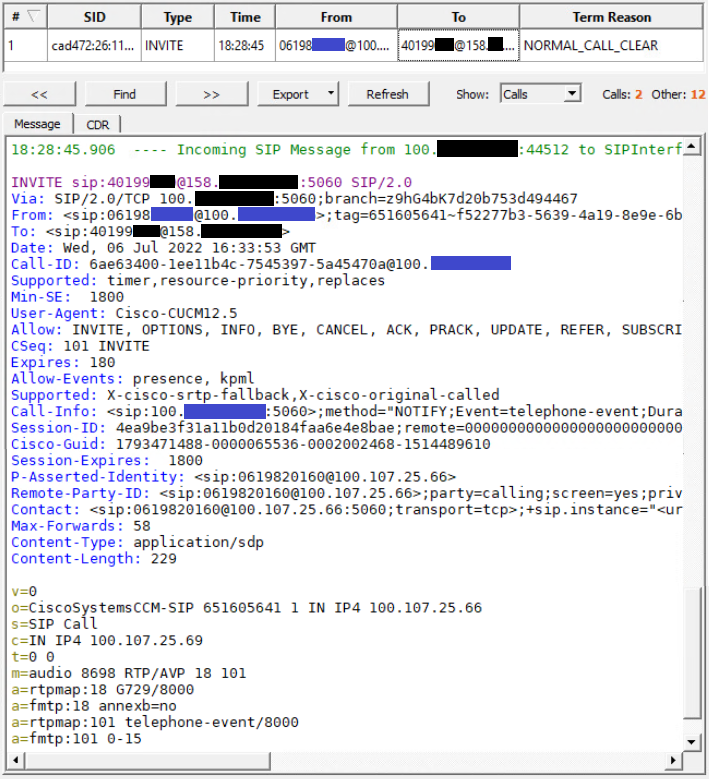
\includegraphics[scale = 0.9]{img/fig_sipflow_param1}
  \caption{Cuerpo del mensaje INVITE inicial}
  \label{figura:fig_sipflow_param1}
\end{figure}

\begin{figure}[h!]
  \centering
  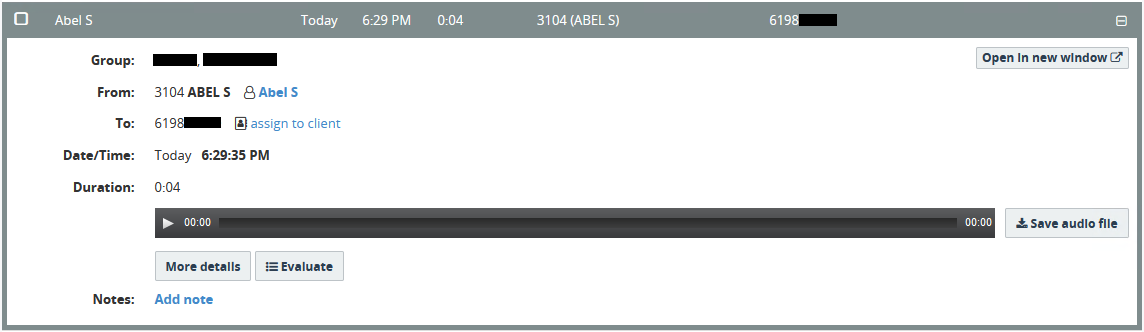
\includegraphics[scale = 0.7]{img/fig_grab_test}
  \caption{Grabación de la llamada de test}
  \label{figura:fig_grab_test}
\end{figure}


%%%%%%%%%%%%%%%%%%%%%%%%%%%%%%%%%%%%%%%%%%%%%%%%%%%%%%%%%%%%%%%%%%%%%%%%%%%%%%%%
%%%%%%%%%%%%%%%%%%%%%%%%%%%%%%%%%%%%%%%%%%%%%%%%%%%%%%%%%%%%%%%%%%%%%%%%%%%%%%%%
% CONCLUSIONES %
%%%%%%%%%%%%%%%%%%%%%%%%%%%%%%%%%%%%%%%%%%%%%%%%%%%%%%%%%%%%%%%%%%%%%%%%%%%%%%%%

\cleardoublepage
\chapter{Conclusiones}
\label{chap:conclusiones}

A pesar de las fechas agresivas que tenía la empresa contratante y de que me hubiera gustado disponer de mayor tiempo para un análisis más detallado de cada aspecto de la solución, este proyecto me ha resultado muy útil y didáctico, pues crea un entorno desde cero con un elemento tan importante como el login de agentes a la plataforma desde fuera de la red local. 

Además ha resultado tener una visualización y diseño muy interesante, actualizado y adaptado al contexto en el que nos encontramos, pues el teletrabajo forma ya parte del día a día de la gente, a diferencia de las condiciones laborales anteriores a la pandemia COVID-19.

Tengo que decir que ya poseía ciertos conocimientos sobre el tema, no he cogido este proyecto sin tener nociones mínimas, pero he aprendido mucho y sobre todo he afianzado conocimientos que no terminaban de encajar en mi cabeza por no haber tenido perfectamente claras las bases sobre las que se sustenta esta tecnología. Gracias a este proyecto y estos nuevos conocimientos adquiridos, estoy convencido de que puedo explorar nuevas alternativas, tanto de diseños innovadores como de integración de elementos de otros fabricantes.

\section{Consecución de objetivos}
\label{sec:consecucion-objetivos}

Al tratarse de un proyecto real, es compromiso de la empresa llevar a buen puerto todos los objetivos, por lo que no hay cabida para el incumplimiento de los contenidos pactados. Sin embargo, sí se puede hacer un análisis de cuáles de ellos fueron los más arduos de conseguir, o dieron problemas.

\begin{enumerate}
  \item Se hicieron unas configuraciones específicas en el marcado DTMF para resolver una incidencia durante la integración en donde la locución no cogía el dígito que se pulsaba cuando daba las opciones. En este caso, tras varios días de investigación, se averiguó que se estaba negociando un Payload Type al inicio de la conversación y luego se recibían distintos tipos por cada extremo, lo cual imposibilitaba la comunicación. La solución fue forzar el DTMF por el lado del CUCM, y en el SBC forzar el transcoding hacia las patas interna y externa, dejando el modo “As is” para el RFC 2833 y se definió el payload type a 0 para que aceptara cualquier tipo entrante. Esto significa que no se modifica el payload entrante en el SBC y se trata tal y como se recibe.
  También se habilitó por el lado del Call Manager, en el Sip Trunk hacia el SBC, el método de señalización DTMF como RFC2833, que originalmente estaba definido como \emph{Out of Band}.
  \item Otro problema que me generó muchos días de investigación y numerosos contactos con el soporte del fabricante fue la transmisión de la música en espera en las llamadas que pasaban por el SBC. Internamente funcionaban sin problemas cuando la llamada se transfería o se ponía en espera entre agentes. Este patrón me condujo a pensar que el problema radicaba en el tratamiento de la señal por parte de este elemento de control de borde. En cierto momento conseguí una solución temporal cuando desde el propio SBC cargué un archivo que se ejecutara como música en espera, sobreescribiendo el que transmitía el Call Manager, sin embargo al cabo de unas horas me reportaron que estaba generando problemas de corte de llamadas. Finalmente y tras mucha investigación y pruebas, dí con un parámetro en el Call Manager que debía habilitarse para solucionar este fallo: \emph{Duplex Streaming Enabled}. Estuve mareando al soporte del fabricante del SBC varios días cuando realmente el problema estaba en otro lado. Los agradecimientos de mi memoria también van dirigidos a ellos.
  \item Se detectaron caídas a los pocos minutos en las llamadas a un cliente en concreto. Haciendo \emph{troubleshooting}, se descubrió se estaban enviando muchas peticiones de INVITE que no debían de existir, por lo que se habilitaron dos parámetros que lo solucionaron: \emph{Early Offer Support for voice and video calls}, que añade un MTP (\emph{Media Termination Point}) para habilitar servicios complementarios en la llamada cuando el dispositivo llamante no es capaz de proveer de toda la información necesaria al Call Manager; y \emph{Send end-receive SDP in mid-call INVITE}, que sirve para evitar que el Call Manager envíe mensajes INVITE a=inactive SDP durante una llamada en espera o en una actualización de un códec a mitad de llamada.
\end{enumerate}

\section{Aplicación de lo aprendido}
\label{sec:aplicacion}

En este proyecto he aplicado muchos conocimientos que disponía de la asignatura de \textbf{Protocolos para la Transmisión de Audio y Vídeo en Internet}, pues de todas las asignaturas que he cursado en mi Grado ésta es la que más útil me ha resultado y de la que he podido extraer más enseñanzas a aplicar en esta solución.

\section{Lecciones aprendidas}
\label{sec:lecciones_aprendidas}

Durante la realización de este proyecto he aprendido a:

\begin{enumerate}
  \item Configurar máquinas virtuales y reservar sus recursos.
  \item Configurar desde cero todos los elementos involucrados en este entorno.
  \item Programar un script para Contact Center.
  \item Configurar un Gateway y un SBC para transcodificación.
  \item Desplegar una Autoridad Certificadora y firmar e instalar certificados.
  \item Instalar un DNS y crear los dominios y traducciones.
  \item Entender mucho más a bajo nivel el funcionamiento de un flujo SIP.
  \item Desplegar una base de datos.
  \item Configurar un proxy.
  \item Enlazar una grabadora a un sistema de colaboración.
  \item Hacer \emph{troubleshooting} de tráfico de voz.
  \item Configurar redundancia geográfica y Alta Disponibilidad de equipos.
  \item Asociar una locución a un puerto que se mantiene en espera.
\end{enumerate}


\section{Trabajos futuros}
\label{sec:trabajos_futuros}

Durante la realización de este proyecto y de forma posterior a su finalización, se me fueron ocurriendo varias posibilidades se podrían desarrollar e implementar en un futuro, o en proyectos de características similares:
\begin{itemize}
  \item Se puede integrar un motor de transcripción de audio en la grabadora, de manera que analice las grabaciones y detecte palabras clave para almacenarlas en una base de datos de forma ordenada y que puedan servir de aplicación para soluciones alternativas de big data. Podrán identificar problemas y quejas habituales de los clientes, recoger sugerencias o detectar patrones interesantes de conducta, tanto de los clientes como de los agentes, y poder actuar en base a esos patrones.
  \item A pesar de que se realizó un salvado del estado de la platforma cuando se finalizaron los cambios, se puede desplegar una máquina que aloje \emph{backups} perdiódicos, pues creando un ``punto de guardado'' se mitigan problemas que puedan suceder y que necesiten hacer marcha atrás en las configuraciones.
  \item Se puede implementar una locución en la finalización de la llamada para recoger la opinión del cliente sobre la atención recibida. Se podría configurar una base de datos (o un csv de excel en su defecto) que almacene el número pulsado por el cliente y exportarla a un software específico para la visualización de datos.
\end{itemize}

%%%%%%%%%%%%%%%%%%%%%%%%%%%%%%%%%%%%%%%%%%%%%%%%%%%%%%%%%%%%%%%%%%%%%%%%%%%%%%%%
%%%%%%%%%%%%%%%%%%%%%%%%%%%%%%%%%%%%%%%%%%%%%%%%%%%%%%%%%%%%%%%%%%%%%%%%%%%%%%%%
% BIBLIOGRAFIA %
%%%%%%%%%%%%%%%%%%%%%%%%%%%%%%%%%%%%%%%%%%%%%%%%%%%%%%%%%%%%%%%%%%%%%%%%%%%%%%%%

\cleardoublepage

% Las siguientes dos instrucciones es todo lo que necesitas
% para incluir las citas en la memoria
\bibliographystyle{abbrv}
\bibliography{memoria}  % memoria.bib es el nombre del fichero que contiene
% las referencias bibliográficas. Abre ese fichero y mira el formato que tiene,
% que se conoce como BibTeX. Hay muchos sitios que exportan referencias en
% formato BibTeX. Prueba a buscar en http://scholar.google.com por referencias
% y verás que lo puedes hacer de manera sencilla.
% Más información:
% http://texblog.org/2014/04/22/using-google-scholar-to-download-bibtex-citations/

\end{document}
